% !TeX spellcheck = en_GB
\documentclass[preprint,authoryear]{elsarticle}
% sudo apt-get install -y texlive-publishers

\usepackage[left]{lineno}
\usepackage[utf8]{inputenc}
\usepackage[T1]{fontenc}
\usepackage{lmodern}
\usepackage{multirow}

\usepackage{lineno,hyperref}
\modulolinenumbers[5]

%\usepackage{hyphenat}
\usepackage[none]{hyphenat}

\usepackage{url}
\usepackage{booktabs}

\usepackage{mathtools}
\usepackage{amssymb}
\usepackage{amsthm}

\usepackage{caption}
\captionsetup{labelfont=bf}
\captionsetup{skip=0pt} % vertical distance from the table or figure


\usepackage{algorithm} % sudo apt-get install -y texlive-science

\usepackage[noend]{algpseudocode}

\usepackage[margin=0.9in]{geometry}

\usepackage[normalem]{ulem}
\usepackage{xcolor}

\newcommand{\Comentar}[1]{\State {\cmmt{#1}}}
\newcommand{\Break}{\State \bf {break}}
\renewcommand{\Return}{\State \bf {return}~}
\renewcommand{\algorithmicensure}{\bf {Parameters:}}

\renewcommand\algorithmicthen{}
\renewcommand\algorithmicdo{}


\algblock{ForEach}{EndFor}
\algblock{ForDownTo}{EndFor}
\algblock{ForTo}{EndFor}

\newcommand{\Block}[1]{\State #1 \{}
\newcommand{\EndBlock}{\State \}}

%----- begin celio
\usepackage{scrextend}
\newcommand{\boldm}[1] {\mathversion{bold}#1\mathversion{normal}}
\newcommand{\round}[1]{\ensuremath{\lfloor#1\rceil}}
\usepackage{setspace}
\usepackage{array}
\usepackage{color, colortbl}
\definecolor{Gray}{gray}{0.9}

\newcommand{\specialcell}[2][c]{%
	\begin{tabular}[#1]{@{}c@{}}#2\end{tabular}}

\usepackage{tikz}
\usetikzlibrary{calc}
\usetikzlibrary{positioning}

\usepackage{pgfplots}

\pgfplotsset{
	compat=1.9,
	myplotstyle/.style={
		legend cell align=left,
		every axis plot/.append style={thick},
		legend style={font=\small,draw=none},
		enlargelimits=0.2,
		legend pos=south east,
		y tick label style={ /pgf/number format/.cd, fixed, fixed zerofill, precision=3, /tikz/.cd, },
		x tick label style={ /pgf/number format/.cd, fixed, fixed zerofill, precision=1, /tikz/.cd, },
		grid=major,		
	},
}

%----- end celio

\journal{Computers \& Operations Research}


\begin{document}


\begin{frontmatter}

\title{Parallel air palletization and tour planning for simultaneous pickup and delivery}

\author{A.C.P.~Mesquita}
\ead{celio@ita.br}

\author{C.A.A.~Sanches\corref{cor1}}
\ead{alonso@ita.br}
\cortext[cor1]{Corresponding author.}

\address {Instituto Tecnol\'{o}gico de Aeron\'{a}utica - DCTA/ITA/IEC\\
Pra\c{c}a Mal. Eduardo Gomes, 50\\
S\~{a}o Jos\'{e} dos Campos - SP - 12.228-900 - Brazil}


\begin{abstract}

In the scenario of aerial pickup and delivery of goods in a distribution network, transport aviation faces risks of cargo unbalancing due to the urgency required for loading for rapid take-off and mission accomplishment, especially in times of crisis, public calamity, client contract short lead times, or any external pressure for immediate take-off. Also, there is no technological assistance to help the load and trip planners with the huge number of demands for transport in each hub.
This enables other risks such as improper delivery, excessive fuel burn, and longer than necessary turn-around time. We contributed by modeling and solving a new problem of planning the loading and routing of an aircraft according to a utility score, weight and balance principles, and fuel consumption in a tour of simultaneous pickup and delivery at intermediate hubs.
This new hard problem, named {\it Air Cargo Load Planning with Routing, Pickup, and Delivery Problem (ACLP+RPDP)}, is mathematically modeled using standardized pallets in fixed positions, obeying the center of gravity constraints, delivering each item to its destination, and minimizing fuel consumption costs.
We also contributed by carrying out multiple experiments with the well-known Ant Colony Optimization on synthetic data based on real data from the {\it Brazilian Air Force}\/ transportation history.
These challenging benchmark instances are made publicly available.
We also created a process-based parallel computing heuristic that quickly finds good solutions for a wide range of problem sizes, an essential contribution as { \color{red} it was the unique method that managed to solve all testing scenarios.}

% Reescrever

\end{abstract}

\begin{keyword}
Air Cargo \sep Air Palletization \sep Weight and Balance \sep Pickup and Delivery \sep Vehicle Routing \sep Parallel computing
\end{keyword}

\end{frontmatter}

\label{sec1}
\section{Introduction}


Air cargo transport involves several sub-problems that are difficult to solve. Recently, \cite[p. 401]{BrandtStefan2019} defined the {\it Air Cargo Load Planning Problem} (ACLPP) as four sub-problems: {\it Aircraft Configuration Problem} (ACP), {\it Build-up Scheduling Problem} (BSP), {\it Air Cargo Palletization Problem} (APP) and {\it Weight and Balance Problem} (WBP). Several aspects were considered in this modeling: characteristics of the items to be transported (dimensions, scores, dangerousness, etc.); types and quantities of {\it unit load devices} (ULDs), commonly called pallets; when these pallets are assembled; how items are allocated to pallets; in which positions these pallets are to be placed; how the total cargo weight is balanced; etc. They also presented a comprehensive bibliographic survey of solving methods that had been developed in different situations.

However, there are still other important challenges in air cargo transport that go beyond the definition of the ACLPP, especially with regard to the flight itinerary and the loading and unloading at each destination (or node) of this travel plan. In this context, at least two more important sub-problems can be considered: pickup and delivery operations at each node, called {\it Simultaneous Pickup and Delivery Problem} (SPDP), and the search for the most profitable route, which is the well-known {\it Traveling Salesman Problem} (TSP), similar to the proposed by \cite{kaspi2019}, where the profit per unit time is defined as the profit gained after completing the tour divided by the total time required to complete the tour.

Considering air cargo transport, Table \ref{tab:sa} lists the main works in the literature and the corresponding sub-problems addressed. We also indicate whether the dimensions of the items were taken into account ({\bf 3D} or {\bf 2D}) and which solution method was used: heuristics ({\bf Heu}), integers ({\bf Int}), or linear programming ({\bf Lin}).

\begin{table}[H]
	\centering
	\caption{Air cargo transport: literature, problems and features}  \label{tab:sa}
	\scriptsize
	\renewcommand{\arraystretch}{1.1} % alturas das linhas
	\begin{tabular}{r|cc|cc|cc|ccc}
		\toprule
		                            & {\bf APP}  & {\bf WBP}  &  {\bf SPDP}   &{\bf TSP}   & {\bf 2D}  & {\bf 3D}  & {\bf Heu}  & {\bf Int}  & {\bf Lin} \\
		\midrule
		\cite{LarsenMikkelsen1979}  & $.$        & $\bigstar$ & $.$          & $.$        & $.$       & $.$       & $\bigstar$ & $.$        &  $.$ \\
		\cite{Brosh1981}  & $.$ & $\bigstar$  & $.$   & $.$ & $.$ & $.$   & $.$  & $.$  &  $\bigstar$ \\
		\cite{Kevin1992}  & $.$ & $\bigstar$  & $.$ & $.$ & $.$ &$.$   & $.$  & $\bigstar$  &  $.$ \\
		\cite{Heidelberg1998}  & $.$ & $\bigstar$  & $.$ & $.$ & $\bigstar$ &$.$   & $\bigstar$  & $.$  &  $.$ \\
		\cite{MongeauBes2003}    & $\bigstar$ & $\bigstar$   & $.$ & $.$ & $.$ & $.$   & $.$  & $\bigstar$  &  $.$ \\
		\cite{fok2004optimizing} & $.$ & $\bigstar$   & $.$ & $.$ & $.$ & $.$   & $.$  & $\bigstar$  &  $.$ \\	
		\cite{Chan2006}  & $\bigstar$ & $.$    & $.$ & $.$ & $.$ & $\bigstar$  & $\bigstar$  & $.$  &  $.$ \\
		\cite{KaluznyBohdanL2009Oalb}  & $.$ & $\bigstar$  & $.$  & $.$ & $\bigstar$ &$.$  & $.$  & $\bigstar$  &  $.$ \\
		\cite{Verstichel2011}   & $.$ & $\bigstar$    & $.$ & $.$ & $.$ & $.$   & $.$  & $\bigstar$  &  $.$ \\
		\cite{MesquitaCunha2011}   & $.$ & $.$    & $\bigstar$ & $.$ & $.$ & $.$   & $\bigstar$  & $.$  &  $.$ \\		
		\cite{Limbourg2012} & $.$ & $\bigstar$  & $.$ & $.$ & $.$ & $.$   & $.$  & $\bigstar$  &  $.$ \\
		
		\cite{kaspi2019} & $.$ & $.$  & $.$ & $\bigstar$ & $.$ & $.$   & $\bigstar$  & $.$  &  $.$ \\
		
		\cite{RoesenerHall2014}  & $\bigstar$ & $\bigstar$  & $.$  & $.$ & $.$ & $\bigstar$   & $.$  & $\bigstar$  &  $.$ \\
		\cite{Vancroonemburg2014}  & $\bigstar$ & $\bigstar$   & $.$ & $.$ & $.$ & $.$   & $.$  & $\bigstar$  &  $.$ \\
		\cite{LurkinSchyns2015} & $.$ & $\bigstar$  & $\bigstar$ & $.$  & $.$ & $.$   & $.$  & $\bigstar$  &  $.$ \\
		\cite{RoesenerBarnes2016}  & $.$ & $\bigstar$   & $.$ & $.$ & $.$ & $.$   & $\bigstar$  & $.$  &  $.$ \\
		\cite{PaquaySchynsLimbourg2016,PaquayLimbourgSchynsOliveira2018}  & $\bigstar$ & $\bigstar$ & $.$ & $.$ & $.$ & $\bigstar$ & $\bigstar$  & $\bigstar$ & $.$ \\
		\cite{YangLiuGao2018} & $.$ & $\bigstar$  & $.$  & $.$ & $\bigstar$  & $.$ & $\bigstar$ & $.$  & $.$ \\
		\cite{wong2020} & $\bigstar$  & $\bigstar$  & $.$  & $.$   & $.$  & $.$ & $.$ & $\bigstar$  & $.$  \\
		\cite{eugene2021} & $\bigstar$ & $\bigstar$ & $.$  & $.$   & $.$ & $.$ & $.$ & $\bigstar$  & $.$  \\
		\cite{zhao2021} & $.$ & $\bigstar$ & $.$  & $.$  & $.$ & $.$ & $.$  & $\bigstar$ &  $.$ \\
		{\bf This work}   & $\bigstar$ & $\bigstar$  & $\bigstar$& $\bigstar$ & $.$ & $.$ & $\bigstar$ & $\bigstar$   &  $.$  \\
		\bottomrule 
	\end{tabular}
	\normalsize 
\end{table}

As can be seen, so far \cite{LurkinSchyns2015} is the only work that simultaneously addresses an air cargo (WBP) and a flight itinerary (PDP) sub-problem. Although it is innovative, strong simplifications were imposed by the authors: in relation to loading, APP was ignored; with regard to routing, it is assumed a pre-defined flight plan restricted to two legs. It is important to note that these authors consider an aircraft with two doors, and the minimization of loading and unloading costs at the intermediate node was modeled through a container sequencing problem. Referring directly to this work, \cite[p. 409]{BrandtStefan2019} comment: {\it However, not even these sub-problems are acceptably solved for real-world problem sizes or the models omit some practically relevant constraints}. 

There are real situations that are much more complex. In this work, we consider a practical case in Brazil, which is the largest economy in Latin America. Due to its dimensions, this country has the largest air market on the continent with $2,499$\/ registered airports, of which $1,911$\/ are private and $588$\/ are public. Although it is an immense distribution network, airlift missions consider 3 to 5 nodes per flight plan. Throughout this work, we address routes with up to 7 nodes, as can be seen in Table \ref{tab:costs} and Figure \ref{fig:nodes}.


\begin{table}[H]
	
	\begin{minipage}{0.05\linewidth}
		
	\end{minipage}\hfill % these two lines must be close to each other
	\begin{minipage}{0.45\linewidth}
		
		\caption{Brazilian airports distances ($km$)}  \label{tab:costs}
		\centering
		
		\footnotesize
		
		\newcolumntype{Y}{>{\centering\arraybackslash}p{0.09\textwidth}}
		\newcolumntype{X}{>{\centering}p{0.09\textwidth}}
		
		\begin{tabular}{X X X X X X X Y}
			\toprule
			Node & $l_0$ & $l_1$ & $l_2$ & $l_3$ & $l_4$ & $l_5$ & $l_6$ \\
			IATA*   & GRU   & GIG   & SSA   & CNF   & CWB   & BSB   & REC \\	
			\midrule	
			GRU     & 0	    &343	&1,439   &504    &358    &866    &2,114\\
			GIG	    & 343	&0	    &1,218   &371    &677    &935    &1,876\\
			SSA	    & 1,439	&1,218	&0	    &938    &1,788   &1,062   &676\\
			CNF	    & 504	&371	&938	&0	    &851    &606    &1,613\\
			CWB	    & 358	&677	&1,788	&851	&0	    &1,084   &2,462\\
			BSB	    & 866	&935	&1,062	&606	&1,084	&0	    &1,658\\
			REC	    & 2,114	&1,876	&676	&1,613	&2,462	&1,658	&0\\
			\bottomrule
			\multicolumn{8}{c}{*International Air Transport Association}\\
			\multicolumn{8}{c}{\small\textsuperscript{Source: www.airportdistancecalculator.com}}\\
		\end{tabular}
		\normalsize
		
	\end{minipage}\hfill % these two lines must be close to each other
	\begin{minipage}{0.50\linewidth}
		\centering
		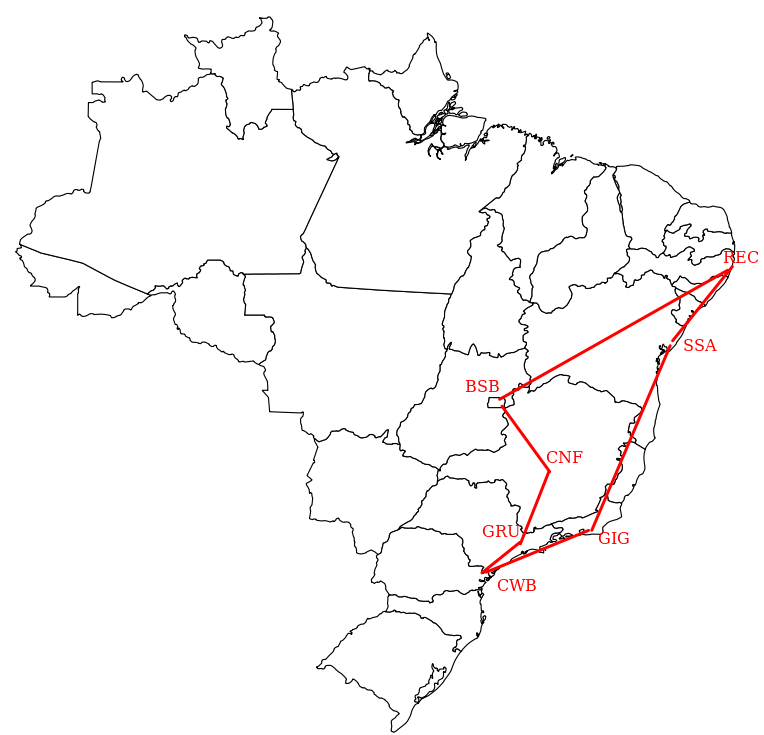
\includegraphics[scale=0.25]{Images/nodes.png}
		\captionof{figure}{A route between Brazilian airports}
		\label{fig:nodes}		
	\end{minipage}
\end{table}


In the {\it Brazilian Air Force}\/ missions, hundreds of items can be carried at each node, where the objectives are to prioritize the transport of the most important items and minimize the cost of fuel along the route. As standardized pallets are used with predefined positions on the aircraft, it is possible to carry out loading and unloading at each node in around two hours. However, there is no technological assistance that guarantees the achievement of these objectives.

This work proposes a method that attends these objectives: a pallet building and arrangement plan with a routing option that maximizes the benefit-cost ratio for the smooth execution of pickup and delivery transport missions. We develop a heuristic that can be executed on a simple handheld computer (like a laptop or a tablet) and that provides a solution quickly enough to keep this cargo handling time under an hour. This heuristic will reduce the stress that transport planners are subjected to, because they have to deal with a lot of information in planning the aircraft route, assembling the pallets, and picking up and delivering at each node. To the best of our knowledge, this is the first time that an air cargo transport problem that simultaneously involves APP, WBP, PDP and TSP has been addressed. This new problem is named {\it Air Cargo Load Planning with Routing, Pickup and Delivery Problem} (ACLP+RPDP).

This article is organized into six more sections. In Section \ref{sec2}, we give a brief review of the literature. In Section \ref{sec3}, we present the problem context and assumptions and, in Section \ref{sec4}, the mathematical model and how we dealt with its issues. In Section \ref{sec5}, we describe the elaborate algorithms, whose results are presented in Section \ref{sec6}. Finally, our conclusions are in Section \ref{sec7}.


\section{Related literature}
\label{sec2}

In this section, we briefly describe the characteristics of the main works related to air cargo transport, following the chronological order of Table \ref{tab:sa}.

\cite{LarsenMikkelsen1979} developed an interactive procedure for loading 14 types of Boeing 747 into a two-leg flight plan. Seven types of items were considered to be allocated in 17 to 42 positions. With non-linear programming and heuristics, they present a solution that minimizes positioning changes in the intermediate node, optimizing the load balancing in the aircraft.

\cite{Brosh1981} addressed the problem of planning the allocation of cargo on an aircraft. Considering volume, weight and structural constraints, the author finds the optimal load layout through a fractional programming problem.

\cite{Kevin1992} developed a multi-criteria optimization approach to load the {\it C-130} aircraft of the {\it Canadian Air Force}. Based on integer programming, this model provides timely planning and improves airlift support for combat operations, solving WBP with pallets in fixed positions, and considering 20 different items.

\cite{Heidelberg1998} developed a heuristic for 2D packing in air loading, comparing it with methods for solving the {\it Bin Packing Problem}. Authors conclude that the classical algorithms are inadequate in this context, because they ignore the aircraft balancing constraints.

\cite{MongeauBes2003} presented a method based on linear integer programming to solve the problem of choosing and positioning containers on the {\it Airbus 340-300}. Safety and stability restrictions were considered, with the objective of minimizing fuel consumption.

\cite{fok2004optimizing} developed a web-based application to make efficient use of space and load balancing for an air cargo company. Based on an analysis of historical data, an operational load planning with mathematical optimization is obtained. This container load planning is usually done roughly 2 hours before departure, when all cargo details are in place.

\cite{Chan2006} carried out a case study with heterogeneous pallets. In order to minimise the total cost of shipping, they developed a 3D packing heuristic, with a loading plan for each pallet. Although the authors do not consider load balancing or positioning of pallets in the cargo hold, this method is relevant in commercial and industrial applications, where cargo items tend to be less dense.

\cite{KaluznyBohdanL2009Oalb} developed a mixed integer linear programming model to arrange a set of items in a military context that optimizes the load balance.

\cite{Verstichel2011} solved WBP by selecting the most profitable subset of containers to be loaded onto an aircraft using mixed-integer programming. Experimental results on real-life data showed significant improvements compared to those obtained manually by an experienced planner.

\cite{MesquitaCunha2011} presented a heuristic for a real problem of the {\it Brazilian Air Force}, which consists of defining transport routes with simultaneous collection and delivery from a central distribution terminal.

\cite{Limbourg2012} developed a mixed-integer program for optimally rearranging a set of pallets into a compartmentalized cargo aircraft, specifically the {\it Boeing 747}.

\cite{kaspi2019} define and solve a new extension of the TSP to maximize the financial contribution per invested time and present an optimal iterative solution procedure for the problem which converges after a limited number of iterations.

\cite{RoesenerHall2014} solved APP and WBP as an integer programming problem, which also allows items to be loaded into pallets according to a specific orientation (e.g., this side up).

\cite{Vancroonemburg2014} presented a mixed integer linear programming model that selects the most profitable pallets, satisfying safety and load balancing constraints on the {\it Boeing 747-400}. Using a solver, authors solved real problems in less than an hour.

As already mentioned, \cite{LurkinSchyns2015} was the first work that simultaneously modeled WBP and SPDP in air cargo transport. The authors demonstrated that this problem is NP-hard and performed some experiments with real data, noting that their model offers better results than those obtained manually.

\cite{RoesenerBarnes2016} proposed a heuristic to solve the {\it Dynamic Airlift Loading Problem} (DALP). Given a set of palletized cargo items that require transport between two nodes in a time frame, the objective of this problem is to select an efficient subset of aircraft, partition the pallets into aircraft loads and assign them to allowable positions on those aircraft.

\cite{PaquaySchynsLimbourg2016} presented a mathematical modeling to optimize the loading of heterogeneous 3D boxes on pallets with a truncated parallelepipeds format. Its objective is to maximise the volume used in containers, considering load balancing restrictions, the presence of fragile items and the possibility of rotating these boxes. \cite{PaquayLimbourgSchynsOliveira2018} developed some heuristics to solve this problem.

\cite{YangLiuGao2018} modeled the air transport problem as a 2D packing problem, and presented a heuristic for its optimization in several aircraft, considering load balancing in order to minimise fuel consumption.

\cite{wong2020}A developed a mathematical model and a tool based on mixed integer programming for optimizing cargo in aircraft with different pallet configurations. Balance restrictions and the presence of dangerous items were considered. \cite{eugene2021} integrated this tool to a digital simulation model, with a visualization and validation system, based on sensors that alert about load deviations.

\cite{zhao2021} proposed a new modeling for WBP based on mixed integer programming. Instead of focusing on the center of gravity (CG) deviation, the authors consider the original CG envelope of the aircraft, with a linearization method for its non-linear constraints.

As can be seen, none of these works address air cargo palletization and load balancing with route optimization in a multi-leg flight plan. This is the objective of our work: to model and elaborate heuristics for a real problem that simultaneously involves 4 intractable sub-problems: APP, WBP, SPDP and TSP.


\section{Problem context and assumptions}
\label{sec3}

In this section, we describe the context of the problem addressed in this work, as well as the assumptions considered.

\subsection{Operational premises}

As we are dealing with an extremely complex and diverse problem, we decided to establish some simplifying characteristics:

\begin{itemize}
	
	\item At each node of the flight plan, the items to be allocated are characterized by weight, volume, scores, and previously known destinations, but do not have dimensions. We leave the consideration of 2D or 3D items for future work.
	
	\item We also disregarded {\it hazardous} items, which eventually could be treated as high score items and other specific constraints.
	
	\item We considered a unique pallet type: the {\it 463L Master Pallet}, a common size platform for bundling and moving air cargo. It is the primary air cargo pallet for more than 70 Air Forces and many air transport companies. This pallet has a capacity of $4500 kg$ and $14.8 m^3$, is equipped for locking into cargo aircraft rail systems, and includes tie-down rings to secure nets and cargo loads, which in total weighs $140 kg$. For more information, see {\tt www.463LPallet.com}.
	
	\item All items allocated on a pallet must have the same destination. A pallet which has not yet reached its destination may receive more items, although it is known that these operations of removing restraining nets increase handling time and the risk of improper delivery. We do not consider oversized cargo in this work, but only cargoes that fit on these pallets.

	\item Finally, as we are interested in minimizing fuel costs while keeping the CG in its operational range, we disregarded some lower ones as handling costs.

\end{itemize}

Throughout this text, we call a {\it consolidated item} a set of items of the same destination stacked on a pallet and covered with a restraining net. It is considered unique, having the same attributes of its components, whose values are the sum of individual scores, weights and volumes. See Figure \ref{fig:larger2}. To ensure accuracy in pickup and delivery operations, consolidated items must remain on board until their destination.


\begin{figure}[H]
	\centering
	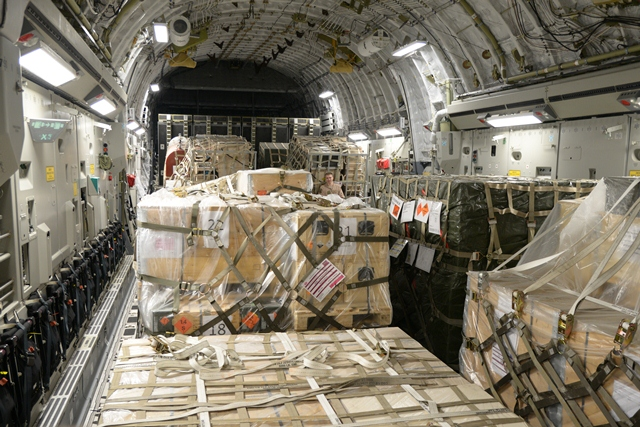
\includegraphics[scale=0.4]{Images/large.png}
	\caption{Consolidated items on pallets inside a {\it Boeing C-17}}
	\small\textsuperscript{Source: https://www.sacprogram.org/en/Pages/Boeing-C-17-Globemaster-III.aspx}
	\label{fig:larger2}
\end{figure}



\subsection{Aircraft and load balancing}


We consider real scenarios with a smaller or a larger aircraft with payloads of $26,000 kg$ or $75,000 kg$ respectively. Both layouts are represented in Figures \ref{fig:smaller} and \ref{fig:larger}, where the pallets are identified by $p_i$.

\begin{figure}[!h]
	\centering
	
	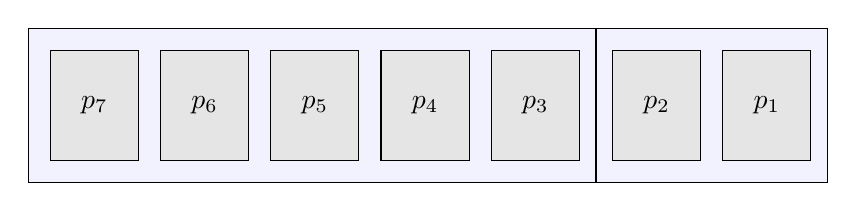
\begin{tikzpicture}[scale=1.4, samples=100]
		
		\filldraw[fill=blue!5!white, draw=black] (0, 0) rectangle (5.15, 1.4);
		\filldraw[fill=gray!20!white, draw=black] (0.2, 0.2) rectangle node{$p_7$} (1.0, 1.2); 
		\filldraw[fill=gray!20!white, draw=black] (1.2, 0.2) rectangle node{$p_6$} (2.0, 1.2); 
		\filldraw[fill=gray!20!white, draw=black] (2.2, 0.2) rectangle node{$p_5$} (3.0, 1.2); 
		\filldraw[fill=gray!20!white, draw=black] (3.2, 0.2) rectangle node{$p_4$} (4.0, 1.2); 
		\filldraw[fill=gray!20!white, draw=black] (4.2, 0.2) rectangle node{$p_3$} (5.0, 1.2); 
		\filldraw[fill=blue!5!white,  draw=black] (5.15,  0) rectangle             (7.25, 1.4);
		\filldraw[fill=gray!20!white, draw=black] (5.3, 0.2) rectangle node{$p_2$} (6.1, 1.2); 
		\filldraw[fill=gray!20!white, draw=black] (6.3, 0.2) rectangle node{$p_1$} (7.1, 1.2);	
		
	\end{tikzpicture}
	
	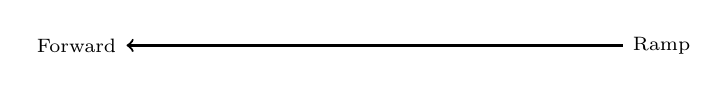
\begin{tikzpicture}[scale=1.4, samples=100]
		\draw[black, thick][<-]  (1, 2.17) node[anchor=east, font=\fontsize{7}{3.5}\selectfont]{Forward} -- (5.5, 2.17) node[anchor=west, font=\fontsize{7}{3.5}\selectfont]{Ramp} ;
	\end{tikzpicture}
	
	\caption{Smaller aircraft layout}
	%\small\textsuperscript{Source: the author}	
	\label{fig:smaller}
\end{figure}



\begin{figure}[!h]
	\centering
	
	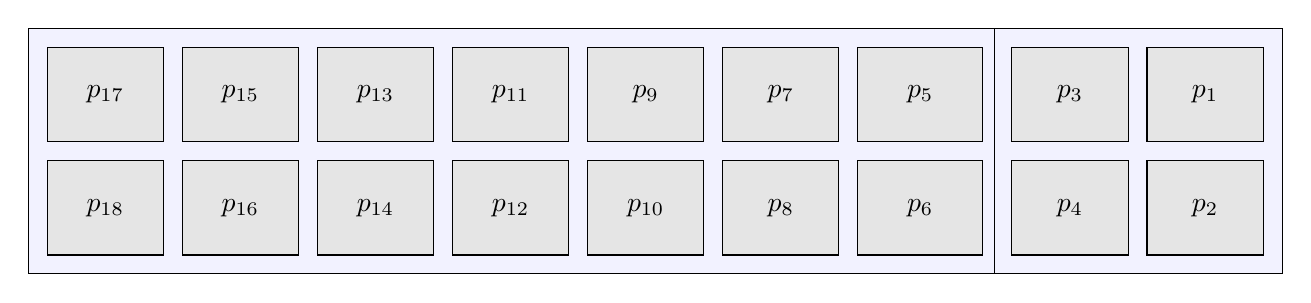
\begin{tikzpicture}[scale=1.2, samples=100]
		
		\filldraw[fill=blue!5!white, draw=black] (0, 0) rectangle (10.23, 2.6);
		
		\filldraw[fill=gray!20!white, draw=black] (0.20, 1.40) rectangle node{$p_{17}$} (1.43, 2.40);
		\filldraw[fill=gray!20!white, draw=black] (0.20, 0.20) rectangle node{$p_{18}$} (1.43, 1.20);
		
		\filldraw[fill=gray!20!white, draw=black] (1.63, 1.40) rectangle node{$p_{15}$} (2.86, 2.40);
		\filldraw[fill=gray!20!white, draw=black] (1.63, 0.20) rectangle node{$p_{16}$} (2.86, 1.20);
		
		\filldraw[fill=gray!20!white, draw=black] (3.06, 1.40) rectangle node{$p_{13}$} (4.29, 2.40);
		\filldraw[fill=gray!20!white, draw=black] (3.06, 0.20) rectangle node{$p_{14}$} (4.29, 1.20);
		
		\filldraw[fill=gray!20!white, draw=black] (4.49, 1.40) rectangle node{$p_{11}$} (5.72, 2.40);
		\filldraw[fill=gray!20!white, draw=black] (4.49, 0.20) rectangle node{$p_{12}$} (5.72, 1.20);
		
		\filldraw[fill=gray!20!white, draw=black] (5.92, 1.40) rectangle node{$p_{9}$} (7.15, 2.40);
		\filldraw[fill=gray!20!white, draw=black] (5.92, 0.20) rectangle node{$p_{10}$} (7.15, 1.20);
		
		\filldraw[fill=gray!20!white, draw=black] (7.35, 1.40) rectangle node{$p_{7}$} (8.58, 2.40);
		\filldraw[fill=gray!20!white, draw=black] (7.35, 0.20) rectangle node{$p_{8}$} (8.58, 1.20);
		
		\filldraw[fill=gray!20!white, draw=black] (8.78, 1.40) rectangle node{$p_{5}$} (10.1, 2.40);
		\filldraw[fill=gray!20!white, draw=black] (8.78, 0.20) rectangle node{$p_{6}$} (10.1, 1.20);
		
		\filldraw[fill=blue!5!white, draw=black] (10.23, 0) rectangle (13.27, 2.6);
		\filldraw[fill=gray!20!white, draw=black] (10.41, 1.40) rectangle node{$p_{3}$} (11.64, 2.40);
		\filldraw[fill=gray!20!white, draw=black] (10.41, 0.20) rectangle node{$p_{4}$} (11.64, 1.20);
		\filldraw[fill=gray!20!white, draw=black] (11.84, 1.40) rectangle node{$p_{1}$} (13.07, 2.40);
		\filldraw[fill=gray!20!white, draw=black] (11.84, 0.20) rectangle node{$p_{2}$} (13.07, 1.20);
		
	\end{tikzpicture}
	
	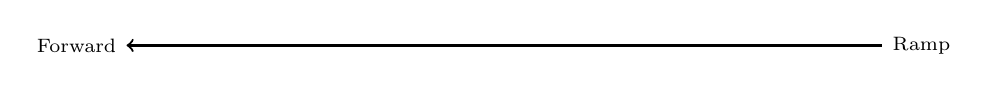
\begin{tikzpicture}[scale=1.2, samples=100]
		\draw[black, thick][<-]  (1, 2.77) node[anchor=east, font=\fontsize{7}{3.5}\selectfont]{Forward} -- (9, 2.77) node[anchor=west, font=\fontsize{7}{3.5}\selectfont]{Ramp} ;
	\end{tikzpicture}
	
	
	\caption{Larger aircraft layout} \label{fig:larger}
\end{figure}


In both cases, the torque applied to the aircraft must keep its CG in the operational range, which corresponds to a percentage of the {\it Mean Aerodynamic Chord} \footnote{Chord is the distance between the leading and trailing edges of the wing, measured parallel to the normal airflow over the wing. The average length of the chord is known as the {\it Mean Aerodynamic Chord} (MAC).}: $0.556m$ in the smaller aircraft and $1.17m$ in the larger one. See Figure \ref{fig:lateral}.

\begin{figure}[H]
	\centering
	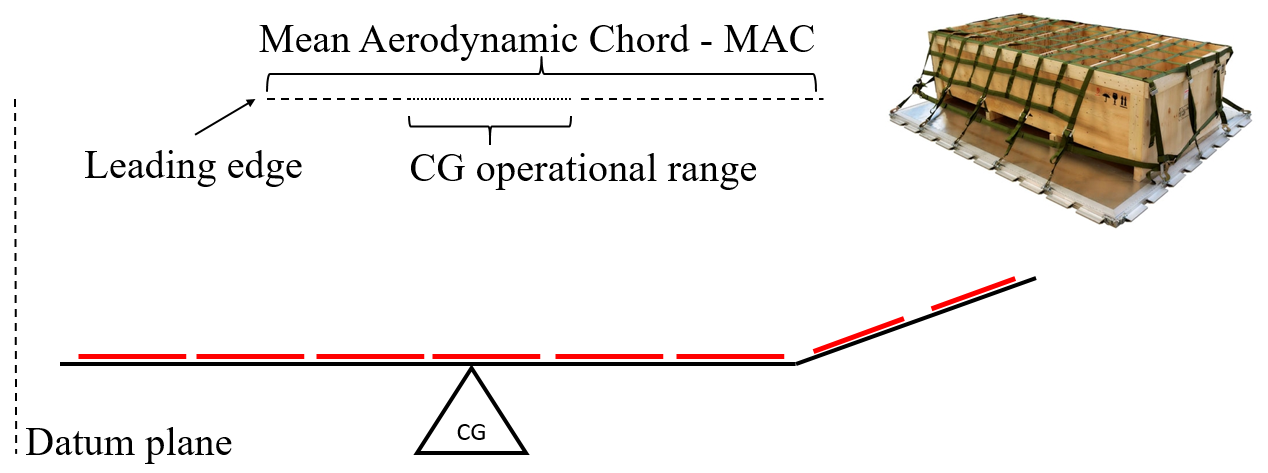
\includegraphics[scale=0.22]{Images/lateral.png}
	\caption{Aircraft longitudinal cut showing red lines as pallets}
	%\small\textsuperscript{Source: the author}
	\label{fig:lateral}
\end{figure}



Tables \ref{tab:smaller} and \ref{tab:larger} show the parameters in both cases. {\it CGx} and {\it CGy} refer to the relative distances of pallet centroids (in meters) in relation to the CG of aircraft along both axes. In both aircraft, as the ramps have an inclination of 25 degrees, we made the necessary corrections in {\it CGx}, {\it Weight} and {\it Volume limits} of the corresponding pallets. The monetary costs of both aircraft are also indicated: per unit of distance in flights between legs ($c_d$) and per deviation in the CG ($c_g$). It is important to consider that $c_g$ tends to zero as the aircraft attitude tends to level.


\begin{table}[H]
	\centering
	\caption{Smaller aircraft parameters}  \label{tab:smaller}
	\footnotesize
	\begin{tabular}{c | c c c c c c c}
		\toprule
		\bf {Limits}  & \multicolumn{3}{c}{$Payload$: $26,000kg$} & \multicolumn{4}{c}{$limit^{CG}_{long}$: $0.556m$} \\
		\midrule
		\bf {Pallets} & $p_7$ & $p_6$ & $p_5$ & $p_4$ & $p_3$ & $p_2$ & $p_1$ \\
		\midrule
		{\bf CGx ($m$)}     & -5.10 & -2.70 & -0.30   & 2.10 & 4.50 & 6.25 & 8.39  \\
		\midrule
		{\bf Weight limits ($kg$)}  & 4,500  &  4,500 &  4,500   & 4,500 & 4,500 & 4,000 & 3,500 \\ 
		{\bf Volume limits ($m^3$)} & 13.7  &  13.7 &  13.7   & 13.7 & 13.7 & 8.9 & 6.9 \\ 
		\midrule

		\bf {Costs}  & \multicolumn{4}{c}{$c_d$: US\$ $1.100/km$ } &	\multicolumn{3}{c}{$c_g = 0.05$} \\

		\bottomrule
	\end{tabular}
	\normalsize 
\end{table}


\begin{table}[H]
	\centering
	\caption{Larger aircraft parameters}  \label{tab:larger}
	\footnotesize
	\begin{tabular}{c | c c c c c c c c c}
		\toprule
		\bf {Limits}& \multicolumn{3}{c}{$Payload$: $75,000kg$} & \multicolumn{3}{c}{$limit^{CG}_{long}$: $1.170m$} &
		\multicolumn{3}{c}{$limit^{CG}_{lat}$: $0.19m$} \\
		\midrule
		\multirow{2}{*}{\bf {Pallets}}  & $p_{17}$ & $p_{15}$ & $p_{13}$ & $p_{11}$ & $p_{9}$ & $p_{7}$ & $p_{5}$ & $p_{3}$ & $p_{1}$ \\
		& $p_{18}$ & $p_{16}$ & $p_{14}$ & $p_{12}$ & $p_{10}$ & $p_{8}$ & $p_{6}$ & $p_{4}$ & $p_{2}$ \\
		\midrule 
		\multirow{2}{*}{\bf {CGx ($m$)}} & -17.57 & -13.17 & -8.77 & -4.40 & 0 & 4.40 & 8.77 & 11.47 & 14.89 \\
		& -17.57 & -13.17 & -8.77 & -4.40 & 0 & 4.40 & 8.77 & 11.47 & 14.89 \\			
		\midrule 
		\multirow{2}{*}{\bf {CGy ($m$)}}  & 1.32 & 1.32 & 1.32 & 1.32 & 1.32 & 1.32 & 1.32 & 1.32 & 1.32 \\
		& -1.32 & -1.32 & -1.32 & -1.32 & -1.32 & -1.32 & -1.32 & -1.32 & -1.32 \\	
		\midrule
		{\bf Weight limits ($kg$)}      &   4,500   &    4,500  &   4,500   &  4,500    & 4,500     & 4,500     & 4,500     & 4,000    & 3,000   \\
		{\bf Volume limits ($m^3$)}   &   14.8   &   14.8   &  14.8    &  14.8    & 14.8     & 14.8     & 14.8     & 10.0    & 7.0 \\	
		\midrule	

		\bf {Costs}  & \multicolumn{5}{c}{ $c_d$: US\$ $4.900/km$ } &	\multicolumn{4}{c}{$c_g = 0.05$} \\

		\bottomrule
	\end{tabular}
	\normalsize 
\end{table}




We also make the following assumptions:
\begin{itemize}
	\item on each pallet, the items are distributed in such a way that their CG coincides with the centroid of the pallet;
	\item the CG of the payload must be at a maximum longitudinal distance of $limit^{CG}_{long}$ from the CG of the aircraft;
	\item in the larger aircraft, the CG of the payload must be at a maximum lateral distance of $limit^{CG}_{lat}$ from the CG of the aircraft;
	\item in the larger aircraft, pallets are distributed in two identical rows (with odd and even indices, respectively), and their centroids are at a distance $d^{CG}_{pallet}$ from the center-line of the aircraft.
\end{itemize}




\subsection{Problem Summary}

\newcolumntype{M}{>{\raggedright}p{0.03\textwidth}}
\newcolumntype{T}{>{\raggedright\arraybackslash}p{0.9\textwidth}}

\bgroup
\def\arraystretch{1.2}
\begin{table}[H]
	\centering
	\small
	\begin{tabular}{MT}
		&Informally, ACLP+RPDP can be summarized as follows:\\
		\midrule
		max &  (items score sum) / (tour cost) of picked up and delivered items on a tour  \\
		\midrule
s.t.    & Along a tour, the set of unvisited nodes is updated. \\
		& In each node, an item may be included in at most one pallet.\\		
		& In each node, consolidated items are composed of items with the same destination. \\
		& Weight, volume and score of a consolidated item are the corresponding sum of their components.\\
		& Consolidated items remain on board until their destinations.\\	
		& Consolidated items can only be included in the same pallet if their destinations are the same.\\
		& Only items destined for the remaining nodes can be loaded.  \\
		& The lateral and longitudinal torques must be within the operational range of the aircraft.\\
		& Weight and volume limitations of pallets must be respected.\\
		& The total weight must be less than the aircraft payload or the total pallet capacity, whichever is the lowest.\\	
		\midrule
	\end{tabular}
	\normalsize
\end{table}
\egroup 



\section{The mathematical modelling}
\label{sec4}

Given the assumptions, scenarios and parameters described in the previous section, we are ready to present the mathematical modeling of ACLP+RPDP, which is one of the contributions of our work.

Let $L = \{ l_0, l_1, \ldots, l_K \}$ be the set of $K+1$ nodes (or destinations), where $l_0$ is the origin and end of a flight plan. Let $d(l_i,l_j)$ be the distance from $l_i$ to $l_j$, where $0 \leq i,j \leq K$. By definition, $d(l_i,l_i)=0$. Let $L_k$ be the set of remaining nodes when the aircraft is in $l_k$, $0 \leq k \leq K$. Therefore, $L_0=L$ and $L_K = \{ l_0 \}$.

Let $C=\{c_{ij}\}$ be the cost matrix of flights, where $c_{ij} = c_d*d(l_i,l_j), 0 \leq i,j \leq K$.

Let $S_K = \{s: \{1, \dots, K\} \rightarrow \{1, \dots, K\} \}$ be the set of $K!$ permutations, which correspond to all possible tours (or itineraries) that have $l_0$ as origin and end, passing through the others $K$ nodes.

Let $M = \{p_1, p_2, \ldots, p_m \}$ the set of $m$ pallets. Each pallet $p_i$, $1 \leq i \leq m$, has weight capacity $p_i.w$, volume capacity $p_i.v$, pallet destinations $p_i.to[k]$, $0 \leq k \leq K$, and distance to the CG of aircraft $p_i.d$. $p_i.to[k]$ denotes that pallet $p_i$ may assume a different destination in each node $k$.

Let $N_k = \{t^k_1, t^k_2, \ldots, t^k_{n_k} \}$ be the set of $n_k$ items to be loaded in node $l_k$, $0 \leq k \leq K$. Each item $t^k_j$, $1 \leq j \leq n_k$, has score $t^k_j.s$, weight $t^k_j.w$, volume $t^k_j.v$, and destination $t^k_j.to \in L_k$. Let $N = \bigcup_{0 \leq k \leq K} N_k$ be the set of items of all nodes along a tour.

Let $Q_k = \{a^k_1, a^k_2, \ldots, a^k_{m_k} \}$ be the set of consolidated items loaded in $m_k \leq m$ pallets when the aircraft arrives at node $l_k$, with $0 \leq k \leq K$. $a^k_i$, $1 \leq i \leq m_k$, is the group of picked-up items that were allocated on pallet $p_i$ in some of the previous nodes. $a^k_i$ has total weight $a^k_i.w$, total volume $a^k_i.v$, and destination $a^k_i.to \in L_k \cup \{l_k\}$. If $a^k_i.to = l_k$, then $a^k_i$ is unloaded, and $p_i$ will be available for reloading; otherwise, $a^k_i$ remains on the aircraft, eventually in another pallet, and with items of $N_k$ having the same destination.

Let $X_{ij}^k$ and $Y_{iq}^k$ be binary variables, where $0 \leq k \leq K$, $1 \leq j \leq n_k$, $1 \leq i \leq m$ and $1 \leq q \leq m_k$. $X_{ij}^k = 1$ if $t_j^k$ is assigned to $p_i$ in node $l_k$, and 0 otherwise. $Y_{iq}^k = 1$ if $a_q^k$ is assigned to $p_i$ in node $l_k$, and 0 otherwise. By definition, $Y_{iq}^0=0$. Allocations of items or consolidated items to pallets in node $l_k$ can be seen as a bipartite graph $G_k(V_k, E_k)$, where $V_k = M \cup N_k \cup Q_k$, $E_k = E^N_k \cup E^Q_k$, $(p_i, t_j^k) \in E^N_k$ if $X_{ij}^k = 1$, and $(p_i, a_q^k) \in E^Q_k$ if $Y_{iq}^k = 1$.

The mathematical modeling of this problem is described in the equations below.


\begin{equation} \label{eq:maxf}
	\max_{\pi \in S_K} f_\pi(\tilde{s},\tilde{c})
\end{equation}

\begin{equation} \label{eq:scores}
	\tilde{s} = \sum_{k=0}^{K} \sum_{i=1}^{m} \sum_{j=1}^{n_k} X_{ij}^k \times t_j^k.s
\end{equation}

\begin{equation} \label{eq:costs}
	\tilde{c} = c_{0,\pi(1)}\times(1+c_g\times|\epsilon_0|) + \sum_{k=1}^{K-1} [ c_{\pi(k), \pi(k+1)}\times(1+c_g\times|\epsilon_k|) ] + c_{\pi(K),0}\times(1+c_g\times|\epsilon_K|)
\end{equation}

\begin{equation} \label{eq:maxW}
	maxW = \min(Payload, \sum_{i=1}^{m}p_i.w)
\end{equation}

\begin{equation} \label{eq:tau}
\tau_k = \sum_{i=1}^{m}[ p_i.d \times (\sum_{j=1}^{n_k} X_{ij}^k \times t_j^k.w +  \sum_{q=1}^{m} Y_{iq}^k \times a_q^k.w)];\ k \in \{0, 1, \ldots, K\}
\end{equation}

\begin{equation} \label{eq:eps}
\epsilon_k = \frac{\tau_k}{maxW \times limit^{CG}_{long}};\ k \in \{0, 1, \ldots, K\}
\end{equation}

\begin{equation} \label{eq:pdp11}
	L_0 = L; L_{k} = L_{k-1} - \{l_{\pi(k)}\}; \ k \in \{1, 2, \ldots, K\}
\end{equation}

\begin{equation} \label{eq:pdp13}
	Y^0_{iq} = 0; a^0_i.w = 0; a^0_i.v = 0; a^0_i.to = -1;\ i,q \in \{1, 2, \ldots, m\}
\end{equation}

\begin{equation} \label{eq:pdp12}
	X_{ij}^k = 0 \ \mbox{if} \ t_j^k.to \notin L_k; \ i \in \{1, 2, \ldots, m\}; \ j \in \{1, 2, \ldots, n_k\}; \ k \in \{1,2, \ldots, K\}
\end{equation}

\begin{equation} \label{eq:pdp9}
	Y_{iq}^k = 0 \ \mbox{if} \ a_i^k.to \notin L_k; \ i \in \{1, 2, \ldots, m\}; \ q \in \{1, 2, \ldots, m_k\}; \ k \in \{ 1, 2, \ldots, K\}
\end{equation}

\begin{equation} \label{eq:cons2}
	a_i^{\pi(k+1)}.w = \sum_{j=1}^{n_k} X_{ij}^{\pi(k)} \times t_j^{\pi(k)}.w + \sum_{q=1}^{m_k} Y_{iq}^{\pi(k)} \times a_q^{\pi(k)}.w;  \ i \in \{1, 2, \ldots, m_k\}; k \in \{0, 1, \ldots, K-1\}
\end{equation}

\begin{equation} \label{eq:cons3}
	a_i^{\pi(k+1)}.v = \sum_{j=1}^{n_k} X_{ij}^{\pi(k)} \times t_j^{\pi(k)}.v + \sum_{q=1}^{m_k} Y_{iq}^{\pi(k)} \times a_q^{\pi(k)}.v;  \ i \in \{1, 2, \ldots, m_k\}; k \in \{0, 1, \ldots, K-1\}
\end{equation}

\begin{equation} \label{eq:cons5}
	a_i^{\pi(k+1)}.to = t^{\pi(k)}_j.to  \ \mbox{if} \ X^{\pi(k)}_{ij} = 1  \ \mbox{and} \ t^{\pi(k)}_j.to \in L_{k+1};  \ i \in \{1, 2, \ldots, m_k\}; \ j \in \{1, 2, \ldots, n_k\}; \ k \in \{0,1, \ldots, K-1\}
\end{equation}

\begin{equation} \label{eq:LatIt}
	LatIt_k = \sum_{i=1}^{m} \sum_{j=1}^{n_k} ( X_{ij}^k \times t_j^k.w \times (i\%2) - X_{ij}^k \times t_j^k.w \times (i+1)\%2 ); \ k \in \{0, 1, \ldots, K\}
\end{equation}

\begin{equation} \label{eq:LatCons}
	LatCons_k =  \sum_{i=1}^{m} \sum_{q=1}^{m_k}  ( Y_{iq}^k \times a_q^k.w \times (i\%2) - Y_{iq}^k \times a_q^k.w \times (i+1)\%2); \ k \in \{0, 1, \ldots, K\}
\end{equation}

\begin{equation} \label{eq:torqlat}
	s.t.: d^{CG}_{pallet} \times | LatIt_k + LatCons_k | \leq  \sum_{i=1}^{m}p_i.w \times limit^{CG}_{lat}; \ k \in \{0, 1, \ldots, K\}
\end{equation}

\begin{equation} \label{eq:torqlong}
	s.t.: |\tau_k| \leq maxW \times limit^{CG}_{long};\ k \in \{0, 1, \ldots, K\}
\end{equation}

\begin{equation} \label{eq:payload}
	s.t.: \sum_{i=1}^{m} (\sum_{j=1}^{n_k} X_{ij}^k \times t_j^k.w + \sum_{q=1}^{m_k} Y_{iq}^k \times a_q^k.w ) \leq maxW; \ k \in \{0, 1, \ldots, K\}
\end{equation}

\begin{equation} \label{eq:app2}
	s.t.: \sum_{j=1}^{n_k} X_{ij}^k \times t_j^k.w + \sum_{q=1}^{m_k} Y_{iq}^k \times a_q^k.w  \leq p_i.w; \ i \in \{1, 2, \ldots, m_k\}; \ k \in \{0, 1, \ldots, K\}
\end{equation}

\begin{equation} \label{eq:app3}
	s.t.: \sum_{j=1}^{n_k} X_{ij}^k \times t_j^k.v + \sum_{q=1}^{m_k} Y_{iq}^k \times a_q^k.v  \leq\ p_i.v; \ i \in \{1, 2, \ldots, m_k\}; \ k \in \{0, 1, \ldots, K\}
\end{equation}

\begin{equation} \label{eq:app4}
	s.t.: \sum_{i=1}^{m} X_{ij}^k \leq 1; \ j \in \{1, 2, \ldots, n_k\}; \ k \in \{0, 1, \ldots, K\}
\end{equation}

\begin{equation} \label{eq:app5}
	s.t.:  Y_{iq}^k = 1 \ \mbox{if} \ a^k_q.to \in L_k; \ q \in \{1, 2, \ldots, m_k\}; \ k \in \{0, 1, \ldots, K\}
\end{equation}

\begin{equation} \label{eq:pdp8}
	s.t.: p_i.to[k] = t^k_j.to\ \mbox{if} \ X_{ij}^k = 1; \ i \in \{1, 2, \ldots, m\}; \ j \in \{1, 2, \ldots, n_k\}; \ k \in \{1, 2, \ldots, K\}
\end{equation}

\begin{equation} \label{eq:pdp2}
	s.t.:  p_i.to[k] = a^k_q.to\ \mbox{if} \ Y_{iq}^k = 1; \ i \in \{1, 2, \ldots, m\};\ q \in \{1, 2, \ldots, m_k\}; \ k \in \{1, 2, \ldots, K\}
\end{equation}


The objective of this problem is to find a permutation $\pi \in S_K$\/ that maximizes the function $f_\pi(\tilde{s},\tilde{c})$ \ref{eq:maxf}. In this way, the flight plan will be $l_0, l_{\pi(1)}, \ldots, l_{\pi(K)}, l_0$. $\tilde{s}$\/ is the total score of transported items \ref{eq:scores} and  $\tilde{c}$\/ is the total cost of fuel consumed \ref{eq:costs}. As can be seen, $\tilde{c}$\/ corresponds to the fuel consumption due to the flights carried out and the CG deviation of the transported cargo. Throughout this work, for simplicity, we use $f=\tilde{s}/\tilde{c}$.

The maximum load will be the minimum between the payload and the capacity supported by the pallets \ref{eq:maxW}. Considering the maximum longitudinal distance allowed for the CG, all torques \ref{eq:tau} and deviations \ref{eq:eps} are calculated.

For each step of the flight plan, the set of unvisited nodes is updated \ref{eq:pdp11}. Although there are no items consolidated at the beginning of the flight plan, we defined these variables for ease of notation \ref{eq:pdp13}. Items destined outside the rest of the flight plan will not be loaded (\ref{eq:pdp12} and \ref{eq:pdp9}).

Consolidated items appear when there are items on the pallets that will not be unloaded on the next node. Its weights \ref{eq:cons2} and volumes \ref{eq:cons3} correspond to all the items that were on the pallet, since all these items have the same destination. On subsequent nodes, consolidated items can be allocated with other items of same destination \ref{eq:cons5}.

Equations \ref{eq:LatIt} and \ref{eq:LatCons} respectively, are applied only to the larger aircraft, and calculate the lateral torques of items and consolidated items loaded in both rows of pallets, whose constraint is described in \ref{eq:torqlat}. Similarly, \ref{eq:torqlong} is the longitudinal torque constraint, which is applied to both aircraft sizes.

The weight limitation of the aircraft must be respected \ref{eq:payload}. The sum of weights \ref{eq:app2} and volumes \ref{eq:app3} in each pallet must not exceed its capacity. Each item is associated with a pallet at most \ref{eq:app4}.

Consolidated items remain on board \ref{eq:app5} until their destinations. At each node, an item (\ref{eq:pdp8}) and a consolidated item (\ref{eq:pdp2}) must only be allocated to a pallet if the destinations are the same.


\section{Resolution strategy}
\label{sec5}

Once the assumptions of this work and the mathematical modeling of the problem are presented, it is easy to see that ACLP+RPDP is NP-hard. In a similar way to \cite[p. 6]{LurkinSchyns2015}, consider the simple case where $K=1$\/ (one leg), $m=2$ (two pallets around the aircraft CG), $2n$\/ sufficiently light items with same scores in $l_0$, and no items in $l_1$. Under these conditions, through polynomial reductions for the {\it Set-Partition Problem}, it is possible to demonstrate that the decision problem associated with ACLP+RPDP is NP-complete.

Real cases are more complex as they have hundreds of different items in each node and involve three intractable sub-problems: APP, WBP and SPDP. Through the mathematical modeling presented in the previous section, we verify that {\it Mixed-Integer Programming}\/ (MIP) is not able to solve these cases in feasible time. Thus, it is necessary to adopt some strategy to find a viable solution, not necessarily optimal, that seeks to maximize the objective function $f$.

Our strategy is based on the fact that, in real cases, $K$\/ is usually small. Specifically, we will consider $K \leq 6$\/ throughout this work, which is a higher value than usual in {\it Brazilian Air Force} missions. As a result, if we have fast node-by-node solutions that allow us to construct a complete tour, we will be able to test all possible $K!$\/ tours and thus select the one that provides the best value for the $f$\/ function.

On the other hand, our tactic will be, at each shipping node, to predefine the destinations of the pallets at that node. In this way, we will reserve a number of pallets proportional to the volume demanded by each destination at the shipping node. We could have used another criterion, but it was observed in the experiments that volume is more constrictive in airlift. Once the destinations of the pallets are defined, we will use serial and multiprocessing heuristics to find the best possible node-by-node solutions. This strategy is summarized in Algorithm \ref{alg:main}.


\begin{algorithm}[H]
	\caption{$ACLP+RPDP (scenario,volume)$}  \label{alg:main}
	\begin{algorithmic}[1]
		\State Let $L, M, C$ be according to $scenario$ \label{main:LMC}
		\State $N \gets ItemsGeneration(scenario,volume)$ \label{main:items}
		\For {each $method$}
			\For {each $\pi \in S_K$} \label{main:loop1}
				\State $f_{\pi} \gets SolveTour(\pi, L, M, C, N, method )$ \label{main:method}
			\EndFor \label{main:loop2}
			\State $answer[scenario,volume,method] \gets \max f$ \label{main:f}
		\EndFor
		\State $ {\bf return}\ answer$
	\end{algorithmic}
\end{algorithm}


In this algorithm, there are six values for the $scenario$\/ parameter, according to Table \ref{tab:scenarios}, which defines $K$, the sets of nodes, the aircraft, the pallets and the costs from Tables \ref{tab:smaller} or \ref{tab:larger} that will be used (line \ref{main:LMC}).


The other parameter $volume$\/ is a value greater than 1, which corresponds, at each node $l_k$, to the ratio between the sum of the volumes of the items ($\sum_{j=1}^{n_k} t^k_j.v$) and the load capacity of the pallets ($\sum_{i=1}^{m} p_i.v$). This parameter is passed to $ItemsGeneration$\/ (line \ref{main:items}), responsible for creating the items to be shipped, which will be presented in the next section (Algorithm \ref{alg:itemsgen}).

$method$\/ corresponds to one of the heuristics that we will present in subsection \ref{methods}. The loop of lines \ref{main:loop1}-\ref{main:loop2} goes through all permutations $\pi$, where the node-by-node resolutions are performed by $SolveTour$, whose result is stored in $f_{\pi}$. The best result among all $K!$\/ tours will be the answer for $scenario$, $volume$\/ and $method$\/ (line \ref{main:f}). 

\vspace{2.0mm}
\begin{table}[H]
	\centering
	\caption{Testing scenarios}  \label{tab:scenarios}
	\begin{tabular}{c c c c }
		\toprule
		{\bf Scenario} & {$K$} & {$L$} & {\bf Aircraft} \\		
		\midrule
		1 & 2    & \{$l_0$, $l_1$, $l_2$\}                                 & smaller \\
		2 & 2    & \{$l_0$, $l_1$, $l_2$\}                                 & larger  \\
		3 & 3    & \{$l_0$, $l_1$, $l_2$, $l_3$\}                          & larger  \\
		4 & 4    & \{$l_0$, $l_1$, $l_2$, $l_3$, $l_4$\}                   & larger  \\
		5 & 5    & \{$l_0$, $l_1$, $l_2$, $l_3$, $l_4$, $l_5$\}            & larger  \\
		6 & 6    & \{$l_0$, $l_1$, $l_2$, $l_3$, $l_4$, $l_5$, $l_6$\}     & larger  \\
		\bottomrule
	\end{tabular}
\end{table}

Next, we will present two subsections: in the first we explain how $SolveTour$ is executed, while in the second we will present the heuristics developed for node-by-node resolutions.


\subsection{SolveTour algorithm}
\label{tour}

In addition to the set of nodes, pallets, costs and items, $SolveTour$, described in Algorithm \ref{alg:tour}, receives the parameter $method$, which corresponds to a heuristic for solving the node-by-node problems, and the parameter $\pi$, which is a permutation that defines the order of visits in this tour.

As we mentioned in the previous section, all tours start and end at $l_0$\/ (lines \ref{tour:pi1}-\ref{tour:pi2}).
After initializing the score and cost values (lines \ref{tour:score}-\ref{tour:cost}), there is a loop for the $K+1$\/ flights (lines \ref{tour:loop1}-\ref{tour:loop2}). Initially we set pallets destination as $-1$\/ (line \ref{tour:-1}). When the aircraft is at node $l_0$, the initial graph $G_1$\/ is empty because it has no consolidated items \ref{tour:g11}. Otherwise, the set $L_k$\/ of remaining nodes is updated (line \ref{tour:lk1}), and $UpdateConsolidated$\/ (line \ref{tour:dest}) returns the set of consolidated items that have not yet reached their destination and remain on board, rearranging them on the pallets to minimize CG deviation. This allocation is stored in graph $G_1$\/ (line \ref{tour:g12}).

In the context of this work, we know that $m>K$, once the aircraft has $7$\/ or $18$\/ pallets and $K\leq 6$, allowing there to be at least one pallet for each node to be visited. $SetPalletsDestination$\/ (line \ref{tour:dest2}) presets the destination of each pallet based on the volume demands of the current node, without changing the pallets destination with consolidated items.

Finally, $SolveNode$\/ includes the edges corresponding to the items shipped at the current node, returning the graph $G_2$\/ (line \ref{tour:node}). The score and the CG deviation of this graph are calculated (line \ref{tour:analyse}) and accumulated (lines \ref{tour:score2}-\ref{tour:cost2}), allowing the final result of this tour (line \ref{tour:f}).

\begin{algorithm}[H]
	\caption{$SolveTour(\pi, L, M, C, N, method)$}  \label{alg:tour}
	
	\begin{algorithmic}[1]
		
		\State $\pi(0) \gets 0$ \label{tour:pi1}
		\State $\pi(K+1) \gets 0$ \label{tour:pi2}
		\State $score \gets 0$ \label{tour:score}
		\State $cost \gets 0$ \label{tour:cost}
		\For {$k\gets0$ to $K$} \label{tour:loop1}		
			\For{$i \gets 1$ to $m$}
				\State $p_i.to[k] \gets -1$ \label{tour:-1}
			\EndFor	
			\If {$k = 0$}
				\State $L_0 \gets L$
				\State Let $G_1(M \cup N_0, \varnothing)$ \label{tour:g11}
			\Else
				\State $L_k \gets L_k - \pi(k)$  \label{tour:lk1}			
				\State $Q_{\pi(k)}, E^Q_{\pi(k)}, M \gets UpdateConsolidated(\pi(k))$ \label{tour:dest}			
				\State Let $G_1(M \cup N_{\pi(k)} \cup Q_{\pi(k)}, E^Q_{\pi(k)})$ \label{tour:g12}
			\EndIf  \label{tour:lk2}	
			\State $M \gets SetPalletsDestination( \pi(k) )$ \label{tour:dest2}		
			\State $G_2 \gets SolveNode(method, \pi(k), G_1)$ \label{tour:node}
			\State $s, \epsilon \gets ScoreAndDeviation(\pi(k), G_2)$ \label{tour:analyse}
			\State $score \gets score + s$ \label{tour:score2}
			\State $cost \gets cost + c_{\pi(k),\pi(k+1)} * (1 + c_g * |\epsilon|)$ \label{tour:cost2} 
		\EndFor  \label{tour:loop2}
		\State $ {\bf return}\ score / cost$ \label{tour:f}
		
	\end{algorithmic}
\end{algorithm}

$UpdateConsolidated$, described in Algorithm \ref{alg:cons}, finds the best allocation for the consolidated items that remain on board. Initially, the set $Q$\/ is created, with the consolidated items that did not reach their destination (lines \ref{cons:remain1}-\ref{cons:remain2}). Then $MinCGDeviation$\/ (line \ref{cons:minCG}) is run through a MIP solver with the equations \ref{eq:torque}, \ref{eq:embarked} and \ref {eq:one}, to relocate the consolidated items on the pallets minimizing torque and ensuring that they all remain on board, one on each pallet. As there are few variables, the MIP solver returns an allocation $E^Q_k$\/ very quickly. Finally, the destination of each pallet with consolidated items is updated (lines \ref{cons:Ybegin}-\ref{cons:Yend}).

\begin{algorithm}[H]
	\caption{$UpdateConsolidated(k)$}  \label{alg:cons}
	\begin{algorithmic}[1]

		\State Let $Q_k  = \{ a^k_1, a^k_2, \ldots, a^k_{m_k} \}$ 
		\State $Q \gets \varnothing$ \label{cons:remain1}
		\For{$q\gets1$ to $m_k$} 
			\If {$a_q^k.to \in L_k$} 
				\State $Q \gets Q \cup \{a_q^k\}$
			\EndIf
		\EndFor	 
		\State $m_k \gets |Q|$ \label{cons:remain2}
		\State $E^Q_k \gets MinCGDeviation(k, Q)$ \label{cons:minCG}
		\For{$i \gets 1$ to $m$} \label{cons:Ybegin}
			\For{$q \gets 1$ to $m_k$}
				\If{$(p_i, a_q^k) \in E^Q_k$} 
					\State $p_i.to[k] \gets a_q^k.to$
				\EndIf
			\EndFor		
		\EndFor \label{cons:Yend}
		\State ${\bf return}\ Q, E^Q_k, M$ 
	\end{algorithmic}
\end{algorithm}




\begin{equation} \label{eq:torque}
	\mbox{minimize}\ | \sum_{i=1}^{m} \sum_{q=1}^{m_k} Y^k_{iq} \times p_i.d \times a_q^k.w |,\ \mbox{where}\ Q  = \{ a^k_1, a^k_2, \ldots, a^k_{m_k} \} 
\end{equation}

\begin{equation} \label{eq:embarked}
	s.t.: \sum_{i=1}^{m} Y^k_{iq} = 1;\ q \in \{1,2,\ldots,m_k\}
\end{equation}

\begin{equation} \label{eq:one}
	s.t.: \sum_{q=1}^{m_k} Y^k_{iq} \leq 1;\ i \in \{1,2,\ldots,m\}
\end{equation}


$SetPalletsDestination$, which set pallets destination not yet defined, is described in Algorithm \ref{alg:dest}. The vectors $vol[0..K]$\/ and $PalCons[0..K]$\/ store the total volume of items and the number of pallets with consolidated items destined for each node, respectively (lines \ref{dest:vector1}-\ref{dest:vector2}). The destinations of each pallet are defined proportionally to the volume of items, regarding the pallets with consolidated items (lines \ref{dest:propor1}-\ref{dest:propor2}). The node with the maximum volume demand defines the destination of any remaining pallets (lines \ref{dest:max1}-\ref{dest:max2}).


\begin{algorithm}[H]
	\caption{$SetPalletsDestination(k)$}  \label{alg:dest}
	\begin{algorithmic}[1]
		
		\For{$x \gets 0$ to $K$} \label{dest:vector1}
			\State $vol[x] \gets 0$ 
			\State $PalCons[x]  \gets 0$
		\EndFor
		\State $max \gets 0$ \label{dest:max}
		\State $total \gets 0$ 

		\For{$j \gets 1$ to $n_k$}
			\State $d \gets t_j^k.to$
			\If {$d \in L_k$} 
				\State $vol[d] \gets vol[d] + t_j^k.v$ 
				\State $total \gets total + t_j^k.v$ 
				\If {$vol[d] > vol[max]$}
					\State $max \gets d$ 
				\EndIf
			\EndIf
		\EndFor
		\For{$q \gets 1$ to $m_k$}
			\State $d \gets a_q^k.to$
			\State $PalCons[d] \gets PalCons[d]+1$
			\If {$d \in L_k$} 
				\State $vol[d] \gets vol[d] + a_q^k.v$
				\State $total \gets total + a_q^k.v$ 
				\If {$vol[d] > vol[max]$}
					\State $max \gets d$ 
				\EndIf
			\EndIf
		\EndFor \label{dest:vector2}
		\For{$x \gets 0$ to $K$} \label{dest:propor1}
			\If {$vol[x] \neq 0$}
				\State $quant \gets \max \{1, \lfloor{ m \times vol[x]/total}\rfloor \}-PalCons[x]$ 
				\State $np \gets 0$
				\For{$i \gets 1$ to $m$}
				
					\If{$np = quant$}
						\State ${\bf break}$
					\EndIf
					\If{$p_i.to[k] = -1$}
						\State $p_i.to[x] \gets x$
						\State $np \gets np + 1$
					\EndIf
				\EndFor
				
			\EndIf 
		\EndFor \label{dest:propor2}
		\For{$i \gets 1$ to $m$} \label{dest:max1}
			\If{$p_i.to[k] = -1$}
				\State $p_i.to[x] \gets max$
			\EndIf
		\EndFor \label{dest:max2}
		\State ${\bf return}\ M$ 
		
	\end{algorithmic}
\end{algorithm}


$ScoreAndDeviation$\/ is described in Algorithm \ref{alg:eval}, which evaluates the allocation graph generated by $SolveNode$, returning the corresponding score and CG deviation. It consists of a loop that goes through all the pallets (lines \ref{eval:loop1}-\ref{eval:loop2}), accumulating the scores (lines \ref{eval:score1}-\ref{eval:score2} ) and the torques (lines \ref{eval:eps1}-\ref{eval:eps2}) of the shipped items, allowing the final calculation of the CG deviation (lines \ref{eval:torque1}-\ref{eval:torque2}).

\begin{algorithm}[H]
	\caption{$ScoreAndDeviation(k, G)$}  \label{alg:eval}
	
	\begin{algorithmic}[1]
		\State Let $G(V_k, E^N_k \cup E^Q_k)$
		\State Let $X_{ij}^k = 1$ if $(p_i, t_j^k) \in E^N_k$, $1 \leq i \leq m$, $1 \leq j \leq n_k$
		\State Let $Y_{iq}^k = 1$ if $(p_i, a_q^k) \in E^Q_k$, $1 \leq i \leq m$, $1 \leq q \leq m_k$
		\State $s \gets 0$
		\State $\tau \gets 0$
		\State $weight \gets 0$
		\For{$i \gets 1$ to $m$}	\label{eval:loop1}
			\State $weight \gets weight + p_i.w$		
			\For{$j \gets 1$ to $n_k$}
				\If{$X_{ij}^k = 1$}
					\State $s \gets s + t_{ij}^k.s$ \label{eval:score1}
					\State $\tau \gets \tau + t_{ij}^k.w * p_i.d$ \label{eval:eps1}
				\EndIf
			\EndFor				
			\For{$q \gets 1$ to $m_k$}
				\If{$Y_{iq}^k = 1$}
					\State $s \gets s + a_{iq}^k.s$   \label{eval:score2}
					\State $\tau \gets \tau + a_{iq}^k.w * p_i.d$  \label{eval:eps2}
				\EndIf
			\EndFor	   \label{eval:loop2}
		\EndFor
		\State $maxWeight \gets \min(Payload, weight)$ \label{eval:torque1}
		\State $maxTorque \gets maxWeight \times limit^{CG}_{long}$
		\State $\epsilon \gets \tau/maxTorque$ \label{eval:torque2}
		\State ${\bf return}\ s, \epsilon$	
	\end{algorithmic}
\end{algorithm}


\subsection{Node-by-node solutions}
\label{methods}


In this subsection we present implementations of $SolveNode(method,k, G)$, where $method$\/ corresponds to a heuristic, $k$\/ is the index of the current node and $G$\/ is the allocation graph of the consolidated items that remain on board at node $l_k$.

An important issue on meta-heuristics is that they are known for the hard work in tuning parameters. For this, when we use the word {\it empirically}\/ throughout the text, we want to say that we accomplished many tests with the hardest instances to fit these values. This does not guarantee best results for all instances, but, on average, overall results are acceptable. Another important observation is that our {\it ACO} implementations were designed based on traditional ideas from the literature \cite{Fidanova2006} and on the experiences learned during tests, plus the special features to process-based parallelism.

To guarantee that performance comparisons are made correctly, our implementations use the same elements described below.

\newcolumntype{C}{>{\raggedright}p{0.19\textwidth}}
\newcolumntype{D}{>{\raggedright\arraybackslash}p{0.81\textwidth}}

\bgroup
\def\arraystretch{1.2}
\begin{table}[H]
	\centering
	\small
	\begin{tabular}{CD}
		
		{\it Data structure:}     & Items, pallets and edges are arrays of \emph{Python} class objects, which are initialized with the same data loaded from text files. \\
		
		{\it Stopping criterion:} & All methods have the same time limit of $0.7$ seconds per node.\\
		
		{\it Common procedures:}  & All methods have the same procedures for: solution printing, pallets destinations and initial parameters setting, solution integrity checking, and the same procedures for selecting and inserting edges.\\

	\end{tabular}
	\normalsize
\end{table}
\egroup

The selection of edges for $E^N_k$\/ uses the {\it edge attractiveness}\/ $\theta^k_{ij}$\/ \ref{eq:edge}, which can be understood as the tendency to allocate the item $t^k_j$\/ to the pallet $p_i$. It is directly proportional to the score, and inversely proportional to the volume and the torque of each item. The 3000 value was empirically set to keep the attractiveness in the range [0, 1], to be compatible with the Ant Colony Optimization pheromone range.

\begin{equation} \label{eq:edge}
	\theta^k_{ij}= \frac{t^k_j.s}{t^k_j.v \times 3000}\times(1-\frac{t^k_j.w\times|p_i.d|}{\max_s\{t^k_s.w\}\times\max_q\{|p_q.d|\}});\ i \in \{1,2,\ldots,m\},\ j \in \{1,2,\ldots,n_k\}
\end{equation} 


We use four types of random selections:
\begin{itemize}
	\item $RandomReal(r_1,r_2)$: randomly selects a real number in $[r_1,r_2]$;
	\item $RandomInt(i_1,i_2)$: randomly selects a integer number in $[i_1,i_2]$;
	\item $Roulette(set)$ biased through $\phi$: selects an element from $set$, where the probability of each element is proportional to the value of a given function $\phi$\/ defined on $set$.
\end{itemize}



We also developed Algorithm \ref{alg:greedy}, which generates a greedy allocation of the items available in node $l_k$, according to the non-ascending order of $\theta^k_{ij}$, and considering the consolidated items already shipped. Edges are included in this allocation as long as they respect feasibility constraints. Furthermore, the volume of each pallet $p_i$\/ cannot exceed $p_i.v \times limit$, where $ 0 < limit \leq 1$\/ is a parameter.

\begin{algorithm}[H]
	\caption{ $Greedy(k, G, limit)$}  \label{alg:greedy}

	\begin{algorithmic}[1]
		\State Let $G(V_k, E^Q_k)$
		\State $E^N_k \gets \varnothing$ 			
		\For{$i \gets 1$ to $m$}
			\State $pv[i] \gets 0$ 		
		\EndFor
		\For{$q \gets 1$ to $m_k$}
			\If{$(p_i, a_q^k) \in E^Q_k$} 
				\State $pv[i] \gets pv[i] + a_q^k.v$ 
			\EndIf		
		\EndFor		
		\For {each $e_{ij}^k$ in non-ascending order of $\theta^k_{ij}$}
			\If{($E^N_k \cup \{e_{ij}^k\}$ is feasible) {\bf and} ($pv[i] \leq p_i.v \times limit$)} 
				\State $E^N_k \gets E^N_k \cup \{e_{ij}^k\}$ 
				\State $pv[i] \gets pv[i] + t_j^k.v$ 	
			\EndIf
		\EndFor
		\State ${\bf return}\ G(V_k, E^N_k \cup E^Q_k)$
		
	\end{algorithmic}
\end{algorithm}

To compare allocation graphs generated by the heuristics, we choose the one that offer a higher associated score, since the CG deviation is limited by the restrictions.

In the pseudo-codes presented below, given an allocation graph $G$\/ for the node $l_k$, $f_s(G)$\/ is equivalent to the score $s$\/ returned by $ScoreAndDeviation(k,G) $, described in Algorithm \ref{alg:eval}.

Below, we present 2 implementations for $SolveNode$: {\it Multiprocess Ant Colony Optimization}\/ ({\it mpACO})  and a new parallel heuristic that we propose called {\it Multiprocess Shims (mpShims)}.

It is important to say that the parallel ACO ({\it pACO}) is a different implementation where employs threads instead of processes to solve each ant solution in parallel (for a detailed information on parallel ACO see \cite{Pedemonte2011}). We chose {\it mpACO} for our approach because of the need to share the pheromone array between ants/processes and the facility to handle the possibility of race condition.


\subsubsection{Multiprocess Ant Colony Optimization (mpACO)}

In ACO \cite{Dorigo1992}, a population of $A$\/ ants performs independent search, where each ant $a$\/ finds its own allocation graph $G^a$. Each edge $e^k_{ij}=(p_i,t^k_j)$\/ has a general attractiveness $ga^k_{ij} = (\tau^k_{ij})^\alpha + (\theta^k_{ij})^\beta$, where $\tau^k_{ij}$\/ is the pheromone of this edge, and $\alpha$\/ and $\beta$\/ are constants. If $e^k_{ij}$\/ is included in $G^a$, ant $a$\/ increases the pheromone $\tau^k_{ij}$. Algorithm \ref{alg:aco} presents this heuristic.

\begin{algorithm}[H] 
	
	\caption{ $SolveNode(mpACO, k, G)$ } \label{alg:aco}
	\begin{algorithmic}[1]
		\State Let $G(V_k, E^Q_k)$
		\State $G^*(V_k, E^{N*}_k \cup E^Q_k) \gets Greedy(k, G, 1)$  \label{aco:greedy}
		\State $G^+(V_k, E^{N+}_k \cup E^Q_k) \gets G^*(V_k,E^{N*}_k \cup E^Q_k)$
		\State $A \gets$ a number of ants or parallel processes to be determined for each iteration \label{aco:ants}
		\State $ga^k_{ij}   \gets 0$, $1 \leq i \leq m$, $1 \leq j \leq n_k$  \label{aco:init1}
		\State $\tau^k_{ij} \gets 1$, $1 \leq i \leq m$, $1 \leq j \leq n_k$   \label{aco:init2}
		\State $\alpha    \gets 1.0$ \label{aco:alpha}
		\State $\beta     \gets 4.0$ \label{aco:beta}
		\State $\rho      \gets 0.2$ \label{aco:rho}
		\State $stagnant \gets 0$
		\While{($stagnant < 3$) {\bf and} ($runtime < 0.7s$)} \label{aco:while}
		
		\State $publish$
		\State $solutions \gets subscribe()$		
		
			\For{$a \gets 1$ to $A$} \label{aco:g1}
				\State $G^a(V_k, E^{Na}_k \cup E^Q_k) \gets G^+(V_k, E^{N+}_k \cup E^Q_k)$
				\State $E \gets \{ (p_i,t^k_j) \mid (p_i,t^k_j) \not\in E^{Na}_k \}$
				\While{$|E| > 0$}
					\State $e \gets Roulette(E)$ biased through $ga^k_{ij}$  \label{aco:roulette}
					\State $E \gets E - \{e\}$		
					\If{$E^{Na}_k \cup \{e\}$ is feasible}
						\State $ E^{Na}_k \gets E^{Na}_k \cup \{e\} $ \label{aco:ant2}
					\EndIf	
				\EndWhile	
				\If{$f_s(G^{a}) > f_s(G^{+})$} \label{aco:gen1}
					\State $G^+(V_k, E^{N+}_k \cup E^Q_k) \gets G^a(V_k, E^{Na}_k \cup E^Q_k)$  \label{aco:gen2}
						\For{each $(p_i,t^k_j) \in E^{N+}_k$}
							\State $\tau^k_{ij} \gets \tau^k_{ij} - \Delta\tau^k_{ij}$ \label{aco:phero1}
							\State $ga^k_{ij} \gets (\tau^k_{ij})^\alpha + (\theta^k_{ij})^\beta$ \label{aco:ga1}
						\EndFor
				\EndIf 
			\EndFor \label{aco:g2}
			\If{$f_s(G^+) > f_s(G^*)$} \label{aco:best1}
				\State $stagnant \gets 0$
				\State $G^*(V_k, E^{N*}_k \cup E^Q_k) \gets G^+(V_k, E^{N+}_k \cup E^Q_k)$
				\For{each $(p_i,t^k_j) \in E^{N*}_k$}
					\State $\tau^k_{ij} \gets (1-\rho)\tau^k_{ij}$ \label{aco:rho1}
					\State $\tau^k_{ij} \gets \tau^k_{ij} + \Delta\tau^k_{ij}$ \label{aco:phero2}
					\State $ga^k_{ij} \gets (\tau^k_{ij})^\alpha + (\theta^k_{ij})^\beta$ \label{aco:ga2}
				\EndFor			
			\Else
				\State $stagnant \gets stagnant + 1$ \label{aco:best2}
			\EndIf
			\For{all $\tau^k_{ij}$} 
				\State $\tau^k_{ij} \gets (1-\rho)\tau^k_{ij}$ \label{aco:rho2}
			\EndFor	
		\EndWhile	
		\State ${\bf return}$ $G^*(V_k, E^{N*}_k \cup E^Q_k)$		
	\end{algorithmic}
\end{algorithm}
	
A greedy solution is obtained in line \ref{aco:greedy}, being initially stored in $G^*$\/ and $G^+$. The number $A$\/ of ants was empirically set to 4 (line \ref{aco:ants}), yielding solutions with a good relation quality/time. The $m \times n_k$\/ matrices $\tau^k_{ij}$ and $ga^k_{ij}$\/ (lines \ref{aco:init1}-\ref{aco:init2}) are used and updated by all ants.

In each generation, $A$\/ ants are created (lines \ref{aco:g1}-\ref{aco:g2}). The number of generations depends on the time limit or stagnation in improving results (line \ref{aco:while}). Each ant $a$\/ elaborates its allocation graph $G^a$, considering the current values of $ga^k_{ij}$. To enforce solution diversification, if $(p_i,t^k_j)$ is included in $G^a$\/ then pheromone $\tau^k_{ij}$\/ is decreased (line \ref{aco:phero1}). Similarly, the values of $ga^k_{ij}$\/ are also updated (line \ref{aco:ga1}), where the exponents $\alpha$\/ and $\beta$\/ were chosen empirically: $\alpha$ was set to 1.0 and $\beta$\/ to $4.0$\/ (lines \ref{aco:alpha}-\ref{aco:beta}). For further explanation, see \cite{DorigoManiezzoColorni1996}. 

The best solution of each generation is stored in $G^+$\/ (lines \ref{aco:gen1}-\ref{aco:gen2}), and the update of $G^*$\/ and the stopping criterion are performed on lines \ref{aco:best1}-\ref{aco:best2}. Each edge $(p_i,t^k_j)$\/ in some solution has its corresponding pheromone updated in a cumulative way (line \ref{aco:phero2}), that is, more pheromone will be given to the most relevant edges, where the increment is defined in \ref{eq:delta_tau}. The same with $ga^k_{ij}$\/ (line \ref{aco:ga2}).

\begin{equation} \label{eq:delta_tau}
	\Delta\tau^k_{ij} = \frac{ ga^k_{ij}\times t^k_j.s }{ A \times t^k_j.v}
\end{equation}

Pheromone $\tau^k_{ij}$\/ evaporates (lines \ref{aco:rho1} and \ref{aco:rho2}), where $\rho$\/ is a evaporation rate, which can be seen as a mechanism that delays premature convergence towards a sub-optimal solution. $\rho$\/ was empirically set to $0.2$\/ (line \ref{aco:rho}). 




\subsubsection{Multiprocess Shims - mpShims}


Finally, we present a new heuristic designed specifically for ACLP+RPDP, which we named \emph{mpShims}. Like in mechanics, shims are collections of spacers to fill gaps, which may be composed of parts with different thicknesses (see Figure \ref{fig:shims}). This strategy is based on a practical observation: usually, subsets of smaller and lighter items are saved for later adjustments to the remaining clearances.


\begin{table}[H]
	
	\begin{minipage}{0.08\linewidth}
		
	\end{minipage}\hfill % these two lines must be close to each other
	\begin{minipage}{0.34\linewidth}
		
		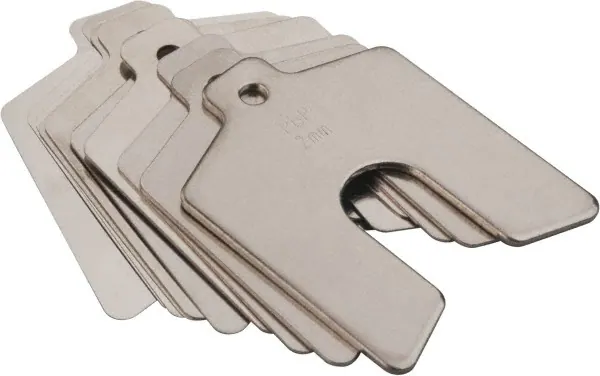
\includegraphics[scale=0.25]{Images/shims.png}
		\captionof{figure}{Shims of various thicknesses}
		\small\textsuperscript{Source: www.mscdirect.com/product/details/70475967}
		\label{fig:shims}
		
	\end{minipage}\hfill % these two lines must be close to each other
	\begin{minipage}{0.58\linewidth}
		
		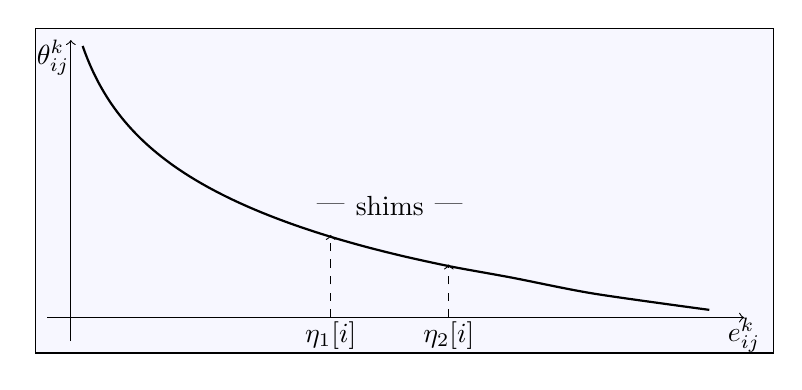
\begin{tikzpicture}[scale=0.75, samples=100]
			\filldraw[fill=blue!3!white, draw=black] (0, 0) rectangle (12.5, 5.5);
			\draw[->] (.2, .6) -- coordinate (x axis mid) (12, .6);
			\node at (5, 0.3) {$\eta_1[i]$};
			\node at (5, 2.5) {|};
			\node at (6, 2.5) {shims};
			\node at (7, 2.5) {|};
			\node at (7, 0.3) {$\eta_2[i]$};
			\node at (0.3, 5) {$\theta_{ij}^k$};
			\draw[->] (.6, .2) -- coordinate (y axis mid) (0.6, 5.3);
			\node at (12, 0.3) {$e_{ij}^k$};
			\draw[smooth, domain = 0.09:2, color=black, thick] plot (.3+1/\x,{4.2+log2(\x)});
			\draw[->, dashed] (5, 0.6)--(5, 2.0);
			\draw[->, dashed] (7, 0.6)--(7, 1.5);
		\end{tikzpicture}
		
		\captionof{figure}{$n_k$\/ edges $e_{ij}^k$\/ of $p_i$\/ sorted by $\theta_{ij}^k$\/ in non-ascending order}
		\label{fig:whip}		
	\end{minipage}
\end{table}


In this heuristic, described in Algorithm \ref{alg:shims}, pallets $p_i$\/ are considered in non-descending order of $|p_i.d|$ (line \ref{shims:pallets}). For each $p_i$, the $n_k$\/ possible edges $e_{ ij}^k$\/ are considered in non-increasing order of $\theta_{ij}^k$\/ (line \ref{shims:edges}) in three phases: the greedy phase (lines \ref{shims:phase1a}-\ref{shims:phase1b}), the composition phase of the shims (lines \ref{shims:phase2a}-\ref{shims:phase2b}) and the selection phase of the best shim (lines \ref{shims:phase3a}-\ref{shims:phase3b}).

Figure \ref{fig:whip} represents the $n_k$\/ possible edges $e_{ij}^k$\/ of $p_i$\/ sorted by $\theta_{ij}^k$. \emph{Shims}\/ starts with a greedy solution, stopping at the edge with index $\eta_1[i]$ close to the local optimum (first phase). Then, considering even the edge with the index $\eta_2[i]$, it elaborates different possible complements for this pallet (second phase) and selects the best of these complements (third phase).

%Examples:
%$\to$ for a small problem if limit is 0.85 for the first phase of the solution process, remains 0.15 for second and third phases.
%$\to$ for a big problem if it is 0.98 for the first phase, it is 0.02 for the remaining phases.




\begin{algorithm}[H]
	\caption{ $SolveNode(Shims, k, G)$}  \label{alg:shims}
	\begin{algorithmic}[1]
		\State Let $G(V_k, E^Q_k)$
		\State Sort $M$ by $|p_i.d|$ in non-descending order \label{shims:pallets}
		\State $E^N_k \gets \varnothing$ 
		\State Let $E[1..m][1..n_k]$, where $E[i]$ is an array with $n_k$ edges $(p_i,t^k_j)$ sorted by $\theta_{ij}^k$ in non-ascending order, $1 \leq i \leq m$ \label{shims:edges}
		\State $gap \gets 2000/n_k*m$ \label{shims:gap} 
		\For{$i \gets 1$ to $m$} 
			\State $pv[i] \gets 0$		\label{shims:phase1a}
			\State $\eta_1[i] \gets 0$
			\While{($p_i.v - pv[i] > gap*p_i.v$) {\bf and} ($\eta_1[i]<n_k$)} \label{shims1:slack}
				\State $\eta_1[i] \gets \eta_1[i] + 1$ \label{shims:eta1}
				\State $e^k_{ij} \gets E[i][\eta_1[i]]$
				\If{($e^k_{ij}$ is feasible) {\bf and} ($t^k_j.v \leq p_i.v - pv[i]$)} 
					\State $E^N_k \gets E^N_k \cup \{e^k_{ij}\}$
					\State $pv[i] \gets pv[i] + t^k_j.v$ 
				\EndIf
			\EndWhile 
			\State $slack[i] \gets p_i.v - pv[i]$
			\State $\eta_2[i] \gets \eta_1[i]$
			\Repeat
				\State $\eta_2[i] \gets \eta_2[i] + 1$  \label{shims:eta2}
				\State $e^k_{ij} \gets E[i][\eta_2[i]]$
				\State $pv[i] \gets pv[i] + t^k_j.v$
			\Until{($\eta_2[i] = n_k$) {\bf or} ($ pv[i] \geq (1 + 3*gap)*p_i.v)$)} \label{shims:phase1b}
			
\State $Set \gets \varnothing$  \label{shims:phase2a}
\State $q \gets 1$
\State $shim[q] \gets \varnothing$
\State $volume \gets 0$
\For{$x \gets \eta_1[i]$ to $\eta_2[i]$}
\State $e_{ij}^k \gets E[i][x]$
\If {($e_{ij}^k \not\in E^N_k \cup shim[q]$) {\bf and} ($e_{ij}^k$ is feasible)}
\If{$t_j^k.v + volume \leq slack[i]$} \label{bincapacity}
\State $shim[q] \gets shim[q] \cup \{e_{ij}^k\}$	
\State $volume \gets volume + t_j^k.v$	
\Else \label{newbins}
\State $Set \gets Set \cup shim[q] $
\State $q \gets q+1$
\State $shim[q] \gets \varnothing$
\State $volume \gets 0$
\If{$t_j^k.v \leq slack[i]$} 
\State $shim[q] \gets shim[q] \cup \{e_{ij}^k\}$	
\State $volume \gets volume + t_j^k.v$
\EndIf
\EndIf
\EndIf
\EndFor   \label{shims:phase2b}
			
			\State $sh_w \gets S$, where $S \in Set$ and $\sum_{e_{ab}^k \in S} t_b^k.w$ is maximum \label{shims:phase3a}
			\State $sh_v \gets S$, where $S \in Set$ and $\sum_{e_{ab}^k \in S} t_b^k.v$ is maximum
			\State $sh_{best} \gets S$, where $S \in \{sh_w, sh_v\}$ and $\sum_{e_{ab}^k \in x} t_b^k.s$ is maximum
			\State $E^N_k \gets E^N_k \cup sh_{best}$ \label{shims:phase3b}
		\EndFor
		\State ${\bf return}$ $G(V_k, E^N_k \cup E^Q_k)$
	\end{algorithmic}
\end{algorithm}

In the first phase (lines \ref{shims:phase1a}-\ref{shims:phase1b}), a greedy and partial solution for $p_i$\/ is constructed by edges inclusion, until a certain slack or clearance is reached. This slack was empirically defined as $gap * p_i.v$\/ (line \ref{shims1:slack}), where $gap = 2000/n_k*m$\/ (line \ref{shims:gap}).

In the second phase (lines \ref{shims:phase2a}-\ref{shims:phase2b}), a set of shims named $Set$\/ is created, where each shim is formed by a group of edges in the range $[\eta_1[i],\eta_2[i]]$, whose total volume is limited by $slack[i]$. In this phase, the heuristic that provided the best results, both in terms of time and quality, is based on {\it Next-Fit}, which is an approximation algorithm for the {\it Bin Packing Problem}\/ \cite{JohnsonGarey1985}. Basically, shims are created by accumulating the following edges, taking $slack[i]$\/ as a limit.

In the third phase (lines \ref{shims:phase3a}-\ref{shims:phase3b}), the best shim in $Set$\/ is chosen. Initially, two shims are found: $sh_w$\/ with larger weight and $sh_v$\/ with larger volume. Among the two, the shim with the highest score will be chosen and its edges are inserted into $E^N_k$.


\section{Implementation and results}
\label{sec6}

This section is composed of two parts: the generation of test instances and the results obtained in our implementations.


\subsection{Instances generation}
\label{items}


As we are dealing with a new problem, which until now had not been modeled in the literature, we have to create our own benchmarks. For this, we based on the characteristics of real airlifts carried out by the {\em Brazilian Air Force}, as described below.

In the military airlift carried out in Brazil from 2008 to 2010, 23\% of the items weighed between $10kg$ and $20kg$, 22\% from $21kg$ to $40kg$, 24\% from $41kg$ to $80kg$, 23\% from $81kg$ to $200kg$, and 8\% between $201kg$ and $340kg$. These five groups of items are described in Table \ref{tab:weights}. On the other hand, the average density of these items is approximately $246 kg/m^3$.

 
\begin{table}[H]
		\centering
		\caption{Items weight distribution ($kg$) in Brazil}  \label{tab:weights}
		\begin{tabular}{c c c c }
			\toprule
			$item$ & $P$ & $low$ & $high$  \\		
			\midrule
			1              & 0.23           & 10  & 20\\
			2              & 0.22           & 21  & 40\\
			3              & 0.24           & 41  & 80 \\		
			4              & 0.23           & 81  & 200\\
			5              & 0.08           & 201 & 340 \\
			\bottomrule
		\end{tabular}
\end{table}


$ItemsGeneration$, which generates $N$, is described in Algorithm \ref{alg:itemsgen}. The parameter $scenario$\/ defines $L$\/ and $M$\/ (line \ref{ig:LM}), and the parameter $volume$\/ sets a limit on the total volume of items at each node (line \ref{ig:extended}). To avoid simply loading all items, we use $volume > 1$.

\begin{algorithm}[H]
	\caption{$ItemsGeneration(scenario,volume)$}  \label{alg:itemsgen}
	\begin{algorithmic}[1]
		\State Let $L$ and $M$ be according to $scenario$ \label{ig:LM}
		\State $limit \gets volume \times \sum_{i=1}^{m} p_i.v$ \label{ig:extended}
		\For{$k \gets 0$ to $K$}
			\State $N_k \gets \varnothing$
			\State $j \gets 0$
			\State $vol \gets 0$	\label{ig:totals}	
			\While{$vol < limit$}
				\State $j \gets j+1$
				\Repeat
					\State $t_j^k.to \gets RandomInt(0, K)$ \label{ig:dest}
				\Until{$t_j^k.to \neq k$}
				\State $x = Roulette(item)$ biased through $P$ \label{ig:weight1}	
				\State $t_j^k.w \gets RandomReal(low(x), high(x))$        \label{ig:weight2}		
				\State $t_j^k.s \gets \round{100 \times (1 - \log_{10}(RandomInt(1, 9)))} $ \label{ig:score}
				\State $t_j^k.v \gets t_j^k.w / RandomReal(148, 344)$ \label{ig:volume}
				\State $vol \gets vol + t_j^k.v$ 
				\State $N_k \gets N_k \cup \{t_j^k\}$ 
			\EndWhile
			\State $n_k \gets j$
		\EndFor
		\State $N \gets \bigcup_{0 \leq k \leq K} N_k$ 
		\State ${\bf return}$ $N$
	\end{algorithmic}
\end{algorithm}

For each generated $t^k_j$\/ item, its destination is uniformly random selected (line \ref{ig:dest}), its weight has a distribution according to Table \ref{tab:weights} (lines \ref{ig:weight1}-\ref{ig:weight2}), its score varies $100$\/ (highest) and $5$\/ (lowest) according to a logarithmic scale (line \ref{ig:score}, and its volume is randomly defined from the density, where we allow a variation of 40\% more or less than the average density of $246 kg/m^3$\/ (line \ref{ig:volume}).



\subsection{Results obtained}


The testing experiments are performed on a 64-bit, 16GiB, 3.2GHz, 8-core processor, 2 threads per core, AMD FX-8320E, with {\it Linux Ubuntu 22.04} as the operational system and {\it Python 3.10.4}\/ as the programming language.

The final experiments are performed on a 64-bit, 128GiB, 3.6GHz, 48-core processor, 2 threads per core, Intel Xeon, with {\it Linux CentOS 8} as the operational system and {\it Python 3.8.2}\/ as the programming language.

For parallelization, we used the {\it Python multiprocessing} package, which implements {\it process-based parallelism} or {\it parallel shared memory algorithm}. According to \cite{multiprocessing}, {\it Multiprocessing} is a package that supports spawning processes using an API similar to the {\it Python Threading} package.

According to \cite[p.271]{Breshears2009}, a {\it Process} is the operating system’s spawned and controlled entity that encapsulates an executing application. A process has two main jobs: the first is to hold the application's resources, and the second is to carry out the application's instructions. 

It is known that working concurrently opens up synchronization issues. But the {\it Multiprocessing} package (mp) offers both local and remote concurrency, effectively side-stepping the global interpreter lock by using sub-processes instead of threads. Because of this, the {\it Multiprocessing} module lets the programmer take full advantage of the fact that a machine has more than one processor, normally capable of 2 threads each.

The decision for {\it Multiprocessing} relies on the need to exchange information among processes (the pheromone trails or some information regarding load balancing, in our case), which would be harder to handle with thread-based parallelism. For this, we used the multiprocessing queue feature that, according to \cite{multiprocessing}, is thread safe.

By Amdahl's law, there is an optimal number of parallel executions for each problem in each environment. While working at IBM in 1967, Gene Amdahl developed the foundation for what became known as Amdahl's Law or Amdahl's Argument. Essentially, the law states that while a process can be decomposed into steps that may then be run in parallel, the time taken for the whole process will be significantly limited by the steps that remain serialized. So, we decided to run some tests to find the best number of parallel processes for each of this work's operational scenarios.

For each red bullet closest to the upper left corner, we call it {\it Utopia}, an impossible result with zero time duration and a possible best score. The blue bullets are experiments performed with the number of parallel processes indicated. The shortest distance from {\it Utopia} may reveal the most efficient parallel processes for the scenario (see Table \ref{tab:scenarios}). 


\begin{figure}[H]
	\begin{center}
		\begin{tikzpicture}[scale=0.8, samples=100]
			\begin{axis}[
				myplotstyle,
				xlabel={\bf mpShims computation times (s)},
				ylabel={\bf Score},
				]
				\addplot+[
				only marks,	
				nodes near coords = {\numProcs{}},
				visualization depends on = {value \thisrow{np} \as \numProcs},						
				]
				table[x=time, y=score, col sep=comma] {./csv/Shims_p1data20.csv};
			\end{axis}
			\fill [red] (canvas cs:x=0.1cm,y=5.6cm) circle (2pt);
		\end{tikzpicture}%
		~%
		%
		\begin{tikzpicture}[scale=0.8, samples=100]
		\begin{axis}[
			myplotstyle,
			xlabel={\bf mpACO computation times (s)},
			ylabel={\bf Score},
			]
			\addplot+[
			only marks,	
			nodes near coords = {\numProcs{}},
			visualization depends on = {value \thisrow{np} \as \numProcs},						
			]
			table[x=time, y=score, col sep=comma] {./csv/ACO_p1data20.csv};
		\end{axis}
		\fill [red] (canvas cs:x=0.1cm,y=5.6cm) circle (2pt);
	\end{tikzpicture}
		
	\end{center}
	\caption{ Scenario 1 performances with $1.2 \times volume$. }
	\label{fig:scenario1data20}
\end{figure}

Observing Figure \ref{fig:scenario1data20}, it may be noticed that the best number of processes for {\it Scenario 1} (the closest to the {\it Utopia}) is \textbf{6}. For {\it Scenario 2}, the best number is \textbf{4}.



\begin{figure}[H]
	\begin{center}
		\begin{tikzpicture}[scale=0.8, samples=100]
			\begin{axis}[
				myplotstyle,
				xlabel={\bf mpShims computation times (s)},
				ylabel={\bf Score},
				]
				\addplot+[
				only marks,	
				nodes near coords = {\numProcs{}},
				visualization depends on = {value \thisrow{np} \as \numProcs},						
				]
				table[x=time, y=score, col sep=comma] {./csv/Shims_p1data50.csv};
			\end{axis}
			\fill [red] (canvas cs:x=0.1cm,y=5.6cm) circle (2pt);
		\end{tikzpicture}%
		~%
		%
		\begin{tikzpicture}[scale=0.8, samples=100]
			\begin{axis}[
				myplotstyle,
				xlabel={\bf mpACO computation times (s)},
				ylabel={\bf Score},
				]
				\addplot+[
				only marks,	
				nodes near coords = {\numProcs{}},
				visualization depends on = {value \thisrow{np} \as \numProcs},						
				]
				table[x=time, y=score, col sep=comma] {./csv/ACO_p1data50.csv};
			\end{axis}
			\fill [red] (canvas cs:x=0.1cm,y=5.6cm) circle (2pt);
		\end{tikzpicture}
		
	\end{center}
	\caption{ Scenario 1 performances with $1.5 \times volume$. }
	\label{fig:scenario1data50}
\end{figure}


\begin{figure}[H]
	\begin{center}
		\begin{tikzpicture}[scale=0.8, samples=100]
			\begin{axis}[
				myplotstyle,
				xlabel={\bf mpShims computation times (s)},
				ylabel={\bf Score},
				]
				\addplot+[
				only marks,	
				nodes near coords = {\numProcs{}},
				visualization depends on = {value \thisrow{np} \as \numProcs},						
				]
				table[x=time, y=score, col sep=comma] {./csv/Shims_p2data20.csv};
			\end{axis}
			\fill [red] (canvas cs:x=0.1cm,y=5.6cm) circle (2pt);
		\end{tikzpicture}%
		~%
		%
		\begin{tikzpicture}[scale=0.8, samples=100]
			\begin{axis}[
				myplotstyle,
				xlabel={\bf mpACO computation times (s)},
				ylabel={\bf Score},
				]
				\addplot+[
				only marks,	
				nodes near coords = {\numProcs{}},
				visualization depends on = {value \thisrow{np} \as \numProcs},						
				]
				table[x=time, y=score, col sep=comma] {./csv/ACO_p2data20.csv};
			\end{axis}
			\fill [red] (canvas cs:x=0.1cm,y=5.6cm) circle (2pt);
		\end{tikzpicture}
		
	\end{center}
	\caption{ Scenario 2 performances with $1.2 \times volume$. }
	\label{fig:scenario2data20}
\end{figure}

\begin{figure}[H]
	\begin{center}
		\begin{tikzpicture}[scale=0.8, samples=100]
			\begin{axis}[
				myplotstyle,
				xlabel={\bf mpShims computation times (s)},
				ylabel={\bf Score},
				]
				\addplot+[
				only marks,	
				nodes near coords = {\numProcs{}},
				visualization depends on = {value \thisrow{np} \as \numProcs},						
				]
				table[x=time, y=score, col sep=comma] {./csv/Shims_p2data50.csv};
			\end{axis}
			\fill [red] (canvas cs:x=0.1cm,y=5.6cm) circle (2pt);
		\end{tikzpicture}%
		~%
		%
		\begin{tikzpicture}[scale=0.8, samples=100]
			\begin{axis}[
				myplotstyle,
				xlabel={\bf mpACO computation times (s)},
				ylabel={\bf Score},
				]
				\addplot+[
				only marks,	
				nodes near coords = {\numProcs{}},
				visualization depends on = {value \thisrow{np} \as \numProcs},						
				]
				table[x=time, y=score, col sep=comma] {./csv/ACO_p2data50.csv};
			\end{axis}
			\fill [red] (canvas cs:x=0.1cm,y=5.6cm) circle (2pt);
		\end{tikzpicture}
		
	\end{center}
	\caption{ Scenario 2 performances with $1.5 \times volume$. }
	\label{fig:scenario2data50}
\end{figure}

%Observing figures \ref{fig:mpShimsdata20}, \ref{fig:mpShimsdata50}, \ref{fig:mpACOdata20}, \ref{fig:mpACOdata50}, it may be noticed that the best overall number of processes for all scenarios is \textbf{?}, because in average it is the number that most of the times is closer to the {\it Utopia} red bullet.



\vspace{2.0mm}

\begin{table}[H]
	\centering
	\caption{Methods and scenarios with $1.2 \times volume$}  \label{tab:20}
%	\footnotesize
\scriptsize
	\begin{tabular}{r|c|c|cccccc|c}
		\toprule
		{$method$}                     &{\bf Procs}              &{\bf Results}     &{\bf 1}     &{\bf 2}    &{\bf 3}      &{\bf 4}      &{\bf 5}      &{\bf 6}     &\specialcell{{\bf Normalized}\\{\bf Speed-up}} \\
		\toprule
	
		
		\multirow{2}{*}{\it {Shims}}   &\multirow{2}{*}{\bf {1}} & $f$              & 5.40        & 2.94    & 2.93         &          &          &         &   \\ 
		                               &                         &{\bf run-time (s)}& <1          & 1       & 4            &            &            &          &   \\ %206s
		\midrule[.1pt]	
		
		\multirow{2}{*}{\it {mpShims}} &\multirow{2}{*}{\bf {?}}& $f$              & 5.88        & 3.16    & 3.16         &          &          &         &   \\ 
		                               &                         &{\bf run-time (s)}& 1           & 10      & 41           &            &            &          &   \\ %299s
		\midrule[.1pt]
		
		\multirow{2}{*}{\it {ACO}}     &\multirow{2}{*}{\bf {1}} & $f$              & 5.77        & 3.49    & 3.02         &        &       &      &   \\ 
                                       &                         &{\bf run-time (s)}& 14          & 808     & 2398          &        &       &      &   \\ 
        \midrule[.1pt]	

        \multirow{2}{*}{\it {mpACO}}   &\multirow{2}{*}{\bf {?}}& $f$              & 5.82        & 3.12    &          &         &       &       &   \\ 
                                       &                         &{\bf run-time (s)}& 22          & 473     &           &         &       &       &   \\ 

        \bottomrule		
	\end{tabular}
	
	\normalsize
	
\end{table}


\section{Conclusions}
\label{sec7}

xxxxx

\section*{Acknowledgments}

This research was partially supported by \textit{S\~{a}o Paulo Research Foundation} (FAPESP, grant 2016/01860-1).

%\bibliographystyle{elsarticle-num} % descomentar antes de submeter
\bibliographystyle{elsarticle-harv} % comentar antes de submeter

%\section*{References}

\bibliography{references}

\end{document}
